% Options for packages loaded elsewhere
\PassOptionsToPackage{unicode}{hyperref}
\PassOptionsToPackage{hyphens}{url}
%
\documentclass[
]{book}
\usepackage{lmodern}
\usepackage{amssymb,amsmath}
\usepackage{ifxetex,ifluatex}
\ifnum 0\ifxetex 1\fi\ifluatex 1\fi=0 % if pdftex
  \usepackage[T1]{fontenc}
  \usepackage[utf8]{inputenc}
  \usepackage{textcomp} % provide euro and other symbols
\else % if luatex or xetex
  \usepackage{unicode-math}
  \defaultfontfeatures{Scale=MatchLowercase}
  \defaultfontfeatures[\rmfamily]{Ligatures=TeX,Scale=1}
\fi
% Use upquote if available, for straight quotes in verbatim environments
\IfFileExists{upquote.sty}{\usepackage{upquote}}{}
\IfFileExists{microtype.sty}{% use microtype if available
  \usepackage[]{microtype}
  \UseMicrotypeSet[protrusion]{basicmath} % disable protrusion for tt fonts
}{}
\makeatletter
\@ifundefined{KOMAClassName}{% if non-KOMA class
  \IfFileExists{parskip.sty}{%
    \usepackage{parskip}
  }{% else
    \setlength{\parindent}{0pt}
    \setlength{\parskip}{6pt plus 2pt minus 1pt}}
}{% if KOMA class
  \KOMAoptions{parskip=half}}
\makeatother
\usepackage{xcolor}
\IfFileExists{xurl.sty}{\usepackage{xurl}}{} % add URL line breaks if available
\IfFileExists{bookmark.sty}{\usepackage{bookmark}}{\usepackage{hyperref}}
\hypersetup{
  pdftitle={Statistics},
  pdfauthor={Dyrehaugen Web Notebook},
  hidelinks,
  pdfcreator={LaTeX via pandoc}}
\urlstyle{same} % disable monospaced font for URLs
\usepackage{longtable,booktabs}
% Correct order of tables after \paragraph or \subparagraph
\usepackage{etoolbox}
\makeatletter
\patchcmd\longtable{\par}{\if@noskipsec\mbox{}\fi\par}{}{}
\makeatother
% Allow footnotes in longtable head/foot
\IfFileExists{footnotehyper.sty}{\usepackage{footnotehyper}}{\usepackage{footnote}}
\makesavenoteenv{longtable}
\usepackage{graphicx}
\makeatletter
\def\maxwidth{\ifdim\Gin@nat@width>\linewidth\linewidth\else\Gin@nat@width\fi}
\def\maxheight{\ifdim\Gin@nat@height>\textheight\textheight\else\Gin@nat@height\fi}
\makeatother
% Scale images if necessary, so that they will not overflow the page
% margins by default, and it is still possible to overwrite the defaults
% using explicit options in \includegraphics[width, height, ...]{}
\setkeys{Gin}{width=\maxwidth,height=\maxheight,keepaspectratio}
% Set default figure placement to htbp
\makeatletter
\def\fps@figure{htbp}
\makeatother
\setlength{\emergencystretch}{3em} % prevent overfull lines
\providecommand{\tightlist}{%
  \setlength{\itemsep}{0pt}\setlength{\parskip}{0pt}}
\setcounter{secnumdepth}{5}
\usepackage{booktabs}
\usepackage{amsthm}
\makeatletter
\def\thm@space@setup{%
  \thm@preskip=8pt plus 2pt minus 4pt
  \thm@postskip=\thm@preskip
}
\makeatother

\renewcommand\chaptername{}
\usepackage[]{natbib}
\bibliographystyle{apalike}

\title{Statistics}
\author{Dyrehaugen Web Notebook}
\date{2022-06-30}

\begin{document}
\maketitle

{
\setcounter{tocdepth}{1}
\tableofcontents
}
\hypertarget{statistics}{%
\chapter{Statistics}\label{statistics}}


\includegraphics{fig/zelda.jpg}

\begin{quote}
The problem with thinking quantitative data and statistics provide proven ``results'' in ``science'' and ``research'' is that you need to be able to obtain precise and accurate data to begin with.
Amid the complexity of real life and inter-related systems, that's nearly impossible.
\end{quote}

\begin{quote}
Most of the things that matter for daily living don't have stationary statistical distributions, unlike games of chance.
Two lessons:
a) don't model everything statistically.
b) if you do model something statistically, don't use a stationary process as your model.
\end{quote}

\begin{quote}
The most important thing about a statistical model is not what it does with the data but what data it uses, and
\end{quote}

\begin{quote}
Often what makes a statistical method useful is that it can make use of more data,
\end{quote}

\begin{quote}
Statistical methods exist within a social context: it's the method and also how it's used.
\end{quote}

\begin{quote}
Pure prediction has fundamental limitations when your goal is to learn about latent properties.
\end{quote}

\hypertarget{probability}{%
\chapter{Probability}\label{probability}}

\hypertarget{intuition-for-probability}{%
\section{Intuition for Probability}\label{intuition-for-probability}}

\emph{Fix}

The human instinct for probability. By most accounts, this instinct is terrible. And that should strike you as odd. As a rule, evolution does not produce glaring flaws. (It slowly removes them.) So if you see flaws everywhere, it's a good sign that you're observing an organism in a foreign environment, a place to which it is not adapted.

When it comes to probability, I argue that humans now live in a foreign environment. But it is of our own creation. Our intuition, I propose, was shaped by observing probability in short samples --- the information gleaned from a single human lifetime. But with the tools of mathematics, we now see probability as what happens in the infinite long run. It's in this foreign mathematical environment that our intuition now lives.

Unsurprisingly, when we compare our intuition to our mathematics, we find a mismatch. But that doesn't mean our intuition is wrong. Perhaps it is just solving a different problem --- one not usually posed by mathematics. Our intuition, I hypothesize, is designed to predict probability in the short run. And on that front, it may be surprisingly accurate.

As a rule, evolutionary biologists don't look for `bias' in animal behavior. That's because they assume that organisms have evolved to fit their environment. When flaws do appear, it's usually because the organism is in a foreign place --- an environment where its adaptations have become liabilities.3

As an example, take a deer's tendency to freeze when struck by headlights. This suicidal flaw is visible because the deer lives in a foreign environment. Deer evolved to have excellent night vision in a world without steel death machines attached to spotlights. In this world, the transition from light to dark happened slowly, so there was no need for fast pupil reflexes. Nor was there a need to flee from bright light. The evolutionary result is that when struck by light, deer freeze until their eyes adjust. It's a perfectly good behavior \ldots{} in a world without cars. In the industrial world, it's a fatal flaw.

Back to humans and our `flawed' intuition for probability. I suspect that many apparent `biases' in our probability intuition stem from a change in our social environment, a change in the way we view `chance'.

\textbf{The gambler's fallacy}

On August 18, 1913, a group of gamblers at the Monte Carlo Casino lost their shirts. It happened at a roulette table, which had racked up a conspicuous streak of blacks. As the streak grew longer, the gamblers became convinced that red was `due'. And yet, with each new roll they were wrong. The streak finally ended after 26 blacks in a row. By then, nearly everyone had gone broke.

These poor folks fell victim to what we now call the gambler's fallacy --- the belief that if an event happens more frequently than normal during the past, it is less likely to happen in the future. It is a `fallacy' because in games like roulette, each event is `independent'. It doesn't matter if a roulette ball landed on black 25 times in a row. On the next toss, the probability of landing on black remains the same (18/37 on a European wheel, or 18/38 on an American wheel).

Many gamblers know that roulette outcomes are independent events, meaning the past cannot affect the future. And yet their intuition consistently tells them the opposite. Gamblers at the Monte Carlo Casino had an overwhelming feeling that after 25 blacks, the ball had to land on red.

The mathematics tell us that this intuition is wrong. So why would evolution give us such a faulty sense of probability?

It is in `games of chance' (like roulette) that flaws in our probability intuition are most apparent. Curiously, it is in these same games where the mathematics of probability are best understood. I doubt this is a coincidence.

The Monte Carlo gamblers who lost their shirts misled by their instinct.
We \emph{recognize} our flaws. We know that our instinct misguides us because we've developed formal tools for understanding probability. Importantly, these tools were forged in the very place where our intuition is faulty --- by studying games of chance.

The crux of the problem. To get an accurate sense for innate probability, you need an absurdly large number of observations. And yet humans typically observe probability in short windows. This mismatch may be why our intuition appears wrong. It's been shaped to predict probability within small samples.

The trouble is, this `long run' is impossibly long.

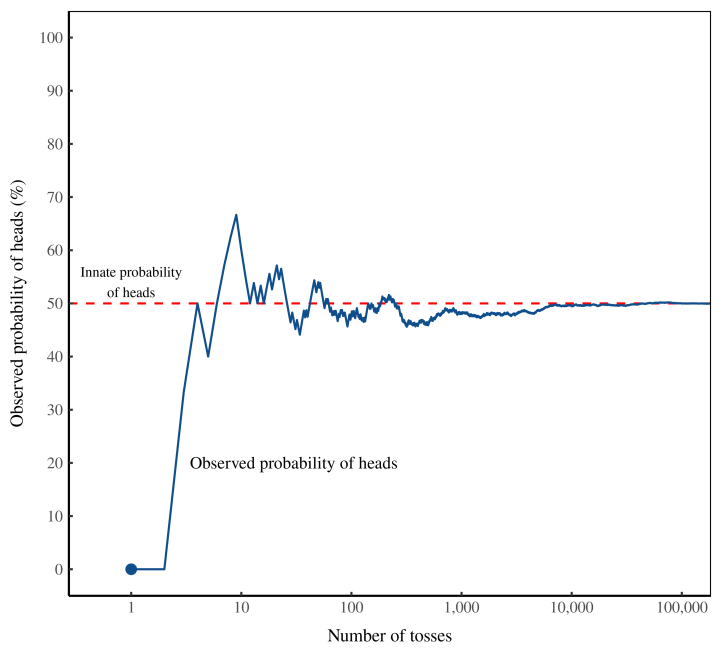
\includegraphics{fig/innate_probability.png}

If observers see a few hundred tosses of the coin, they will deduce the wrong probability of heads.
Even after a few thousand tosses, observers will be misled. In this simulation, it takes about 100,000 tosses before the `observed' probability converges (with reasonable accuracy) to the `innate' probability.

Few people observe 100,000 tosses of a real coin. And that means their experience can mislead. They may conclude that a coin is `biased' when it is actually not. Nassim Nicholas Taleb calls this mistake getting \href{https://en.wikipedia.org/wiki/Fooled_by_Randomness}{`fooled by randomness'}.

For outcomes that were frequent, we could develop an accurate intuition. We are excellent, for instance, at using facial expressions to judge emotions --- obviously because such judgment is a ubiquitous part of social life. But for outcomes that were rare (things like droughts and floods), patterns would be nearly impossible to see.

As a social species, our most significant interactions are with things that do have a memory (i.e.~other humans). So a good rule of thumb may be to project memory onto everything with which we interact.

It could be that our probability intuition is not actually flawed, but is instead a correct interpretation of the evidence \ldots{} as we see it.

Remember that our intuition has no access to the god's eye view of `innate' probability. Our intuition evolved based only on what our ancestors observed. What's important is that humans typically observe probability in short windows. (For instance, we watch a few dozen tosses of a coin.) Interestingly, over these short windows, independent random events \emph{do} have a memory. Or so it appears.

In his article \href{https://jasoncollins.blog/arent-we-smart-fellow-behavioural-scientists/}{`Aren't we smart, fellow behavioural scientists'}, Jason Collins shows you how to give a coin a `memory'. Just toss it 3 times and watch what follows a heads. Repeat this experiment over and over, and you'll conclude that the coin has a memory. After a heads, the coin is more likely to return a tails.

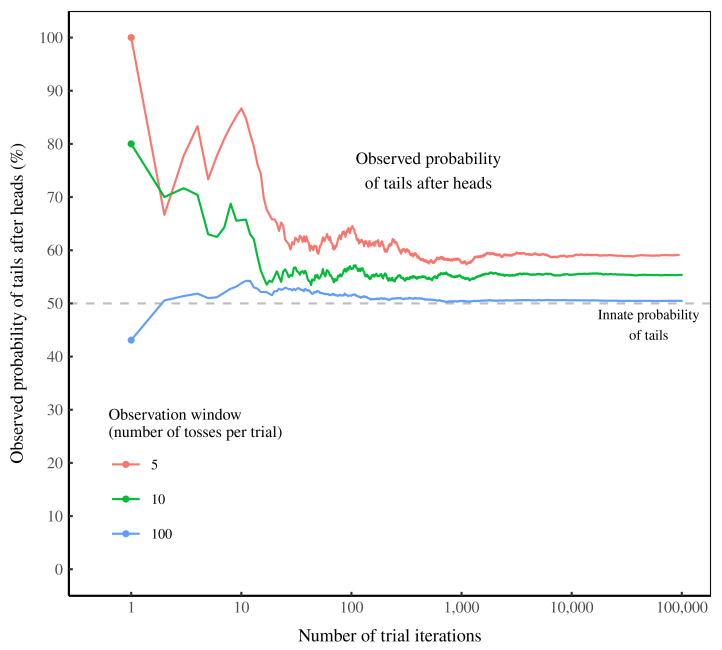
\includegraphics{fig/tails_after_head_by_multi_tosses.png}

The data shouts at us that the coin has a `memory'. Yet we know this is impossible. What's happening?
The coin's apparent `memory' is actually an artifact of our observation window of 3 tosses. As we lengthen this window, the coin's memory disappears.

Here's the take-home message. If you flip a coin a few times (and do this repeatedly), the evidence will suggest that the coin has a `memory'. Increase your observation window, though, and the `memory' will disappear.

When the sample size is small, assuming the coin has a memory is a good way to make predictions.

So what is the evolutionary context of our probability intuition? It is random events viewed through a limited window --- the length of a human life. In this context, it's not clear that our probability intuition is actually biased.

Yes, we tend to project `memory' onto random events that are actually independent. And yet when the sample size is small, projecting memory on these events is actually a good way to make predictions.

\href{https://economicsfromthetopdown.com/2021/07/09/is-human-probability-intuition-actually-biased/}{Fix (2021) Is Human Probability Intuition Actually `Biased'?}

\hypertarget{pandemic-risk-management}{%
\section{Pandemic Risk Management}\label{pandemic-risk-management}}

\emph{Non-Ergodic}

\emph{Paranoia or Nothing}

Taleb and collegues have som very interesting methodological
remarks in the early stages of the COVID-19 outbreak:

\begin{quote}
Clearly, we are dealing with an extreme fat-tailed process
owing to an increased connectivity, which increases the
spreading in a nonlinear way. Fat tailed processes
have special attributes, making conventional risk-management
approaches inadequate
\end{quote}

\begin{quote}
The general (non-naive) precautionary principle delin-
eates conditions where actions must be taken to reduce risk
of ruin, and traditional cost-benefit analyses must not be used.
These are ruin problems where, over time, exposure to tail
events leads to a certain eventual extinction. While there
is a very high probability for humanity surviving a single
such event, over time, there is eventually zero probability of
surviving repeated exposures to such events. While repeated
risks can be taken by individuals with a limited life expectancy,
ruin exposures must never be taken at the systemic and
collective level. In technical terms, the precautionary principle
applies when traditional statistical averages are invalid because
risks are not ergodic.
\end{quote}

\begin{quote}
Historically based estimates of spreading
rates for pandemics in general, and for the current one in
particular, underestimate the rate of spread because of the
rapid increases in transportation connectivity over recent years.
This means that expectations of the extent of harm are under-
estimates both because events are inherently fat tailed, and
because the tail is becoming fatter as connectivity increases
\end{quote}

\begin{quote}
Estimates of the virus's reproductive
ratio \(R\_{0}\) ---the number of cases one case generates on average
over the course of its infectious period in an otherwise
uninfected population---are biased downwards. This property
comes from fat-tailedness due to individual `superspreader'
events. Simply,\(R\_{0}\) is estimated from an average which takes
longer to converge as it is itself a fat-tailed variable.
\end{quote}

\href{https://necsi.edu/systemic-risk-of-pandemic-via-novel-pathogens-coronavirus-\%20a-note}{Norman/Bar-Yam/Taleb Note}
\href{/pdf/Joseph_Norman_2020_Systemic_Risk_of_Pandemic_via_Novel_Pathogenes.pdf}{(pdf)}

\hypertarget{big-data-paradox}{%
\chapter{Big Data Paradox}\label{big-data-paradox}}

\emph{Bradley Abstract}

Surveys are a crucial tool for understanding public opinion and behaviour, and their accuracy depends on maintaining statistical representativeness of their target populations by minimizing biases from all sources. Increasing data size shrinks confidence intervals but magnifies the effect of survey bias: an instance of the Big Data Paradox1. Here we demonstrate this paradox in estimates of first-dose COVID-19 vaccine uptake in US adults from 9 January to 19 May 2021 from two large surveys: Delphi--Facebook2,3 (about 250,000 responses per week) and Census Household Pulse4 (about 75,000 every two weeks). In May 2021, Delphi--Facebook overestimated uptake by 17 percentage points (14--20 percentage points with 5\% benchmark imprecision) and Census Household Pulse by 14 (11--17 percentage points with 5\% benchmark imprecision), compared to a retroactively updated benchmark the Centers for Disease Control and Prevention published on 26 May 2021. Moreover, their large sample sizes led to miniscule margins of error on the incorrect estimates. By contrast, an Axios--Ipsos online panel5 with about 1,000 responses per week following survey research best practices6 provided reliable estimates and uncertainty quantification. We decompose observed error using a recent analytic framework1 to explain the inaccuracy in the three surveys. We then analyse the implications for vaccine hesitancy and willingness. We show how a survey of 250,000 respondents can produce an estimate of the population mean that is no more accurate than an estimate from a simple random sample of size 10. Our central message is that data quality matters more than data quantity, and that compensating the former with the latter is a mathematically provable losing proposition.

\href{https://www.nature.com/articles/s41586-021-04198-4}{Bradley (2021) Unrepresentative big surveys significantly overestimated US vaccine uptake}

\hypertarget{quarantine-fatigue-thins-fat-tailed-impacts}{%
\section{Quarantine fatigue thins fat-tailed impacts}\label{quarantine-fatigue-thins-fat-tailed-impacts}}

\emph{Abstract Conte:}

Fat-tailed damages across disease outbreaks limit the
ability to learn and prepare for future outbreaks,
as the central limit theorem slows down and fails
to hold with infinite moments.

We demonstrate the emergence and persistence of fat tails in contacts across the U.S.
We then demonstrate an interaction between these contact rate distributions
and community-specific disease dynamics
to create fat-tailed distributions of COVID-19 impacts
(proxied by weekly cumulative cases and deaths) during the
exact time when attempts at suppression were most intense.

Our stochastic SIR model implies the effective reproductive number
also follows a fat-tailed stochastic process and leads to multiple waves of
cases with unpredictable timing and magnitude instead of a single noisy wave of cases
found in many compartmental models
that introduce stochasticity via an additively-separable error term.

Public health policies developed based on experiences during these months
could be viewed as an overreaction if these impacts were
mistakenly perceived as thin tailed,
possibly contributing to reduced compliance, regulation, and the quarantine fatigue.

While fat-tailed contact rates associated with superspreaders increase transmission
and case numbers, they also suggest a potential benefit: targeted policy
interventions are more effective than they would be with thin-tailed contacts.

If policy makers have access to the necessary information and a mandate to act decisively,
they might take advantage of fat-tailed contacts
to prevent inaction that normalizes case and death counts that
would seem extreme early in the outbreak.

Our place-based estimates of contacts aid in these efforts by showing
the dynamic nature of movement through communities as the outbreak progresses,
which is quite costly to achieve in network models,
forcing the assumption of static contact networks in many models.

In extreme value theory, fat tails confound efforts to prepare for future extreme events
like natural disasters and violent conflicts because
experience does not provide reliable information about future tail draws.
However, impacts of extreme events play out over time based on policy and
behavioral responses to the event,
which are themselves dynamically informed by past experiences.

A general pattern of fat-tailed contact rate distributions across the U.S.
suggests that fat tails in U.S. cases observed early in the outbreak
are due to city- and county-specific contact networks and epidemiological dynamics.

By unpacking the dynamics that lead to the impacts of extreme events, we show that
1) fat-tailed impacts can also confound efforts to control and manage impacts
in the midst of extreme events and
2) thin tails in disease impacts are not necessarily desirable,
if they indicate an inevitable catastrophe.

\href{https://www.medrxiv.org/content/10.1101/2021.01.07.21249366v1}{Conte (2021) Quarantine fatigue thins fat-tailed coronavirus impacts}
\href{pdf/Conte_2021_Fat-tailed_Corona.pdf}{(pdf)}
\href{pdf/Conte_2021_Fat-tailed_Corona_SM.pdf}{(pdf - SM)}

\hypertarget{herd-immunity-impossible-with-new-mutants}{%
\section{Herd Immunity impossible with new Mutants}\label{herd-immunity-impossible-with-new-mutants}}

Professor of vaccinology Shabir Madhi at the University of the Witwatersrand says protecting at-risk individuals against severe Covid is more important than herd immunity

Leading vaccine scientists are calling for a rethink of the goals of vaccination programmes, saying that herd immunity through vaccination is unlikely to be possible because of the emergence of variants like that in South Africa.

The comments came as the University of Oxford and AstraZeneca acknowledged that their vaccine will not protect people against mild to moderate Covid illness caused by the South African variant.

Novavax and Janssen, which were trialled there in recent months and were found to have much reduced protection against the variant -- at about 60\%. Pfizer/BioNTech and Moderna have also said the variant affects the efficacy of their vaccines, although on the basis of lab studies only.

These findings recalibrate thinking about how to approach the pandemic virus and shift the focus from the goal of herd immunity against transmission to the protection of all at-risk individuals in the population against severe disease.

We probably need to switch to protecting the vulnerable, with the best vaccines we have which, although they don't stop infection, they probably do stop you dying.

\href{https://www.theguardian.com/society/2021/feb/07/scientists-call-for-rethink-as-doubts-grow-about-achieving-herd-immunity}{Vaccine vs New Mutants (Guardian)}

\hypertarget{danish-mask-study}{%
\section{Danish Mask Study}\label{danish-mask-study}}

Every study needs its own statistical tools, adapted to the specific problem, which is why it is a good practice to require that statisticians come from mathematical probability rather than some software-cookbook school. When one uses canned software statistics adapted to regular medicine (say, cardiology), one is bound to make severe mistakes when it comes to epidemiological problems in the tails or ones where there is a measurement error. The authors of the study discussed below (The Danish Mask Study) both missed the effect of false positive noise on sample size and a central statistical signal from a divergence in PCR results.
\textbf{A correct computation of the odds ratio shows a massive risk reduction coming from masks.}

The article by Bundgaard et al., {[}``Effectiveness of Adding a Mask Recommendation to Other Public Health Measures to Prevent SARS-CoV-2 Infection in Danish Mask Wearers'', Annals of Internal Medicine (henceforth the ``Danish Mask Study''){]} relies on the standard methods of randomized control trials to establish the difference between the rate of infections of people wearing masks outside the house v.s. those who don't (the control group), everything else maintained constant.
The authors claimed that they calibrated their sample size to compute a p-value (alas) off a base rate of 2\% infection in the general population.
The result is a small difference in the rate of infection in favor of masks (2.1\% vs 1.8\%, or 42/2392 vs.~53/2470), deemed by the authors as not sufficient to warrant a conclusion about the effectiveness of masks.

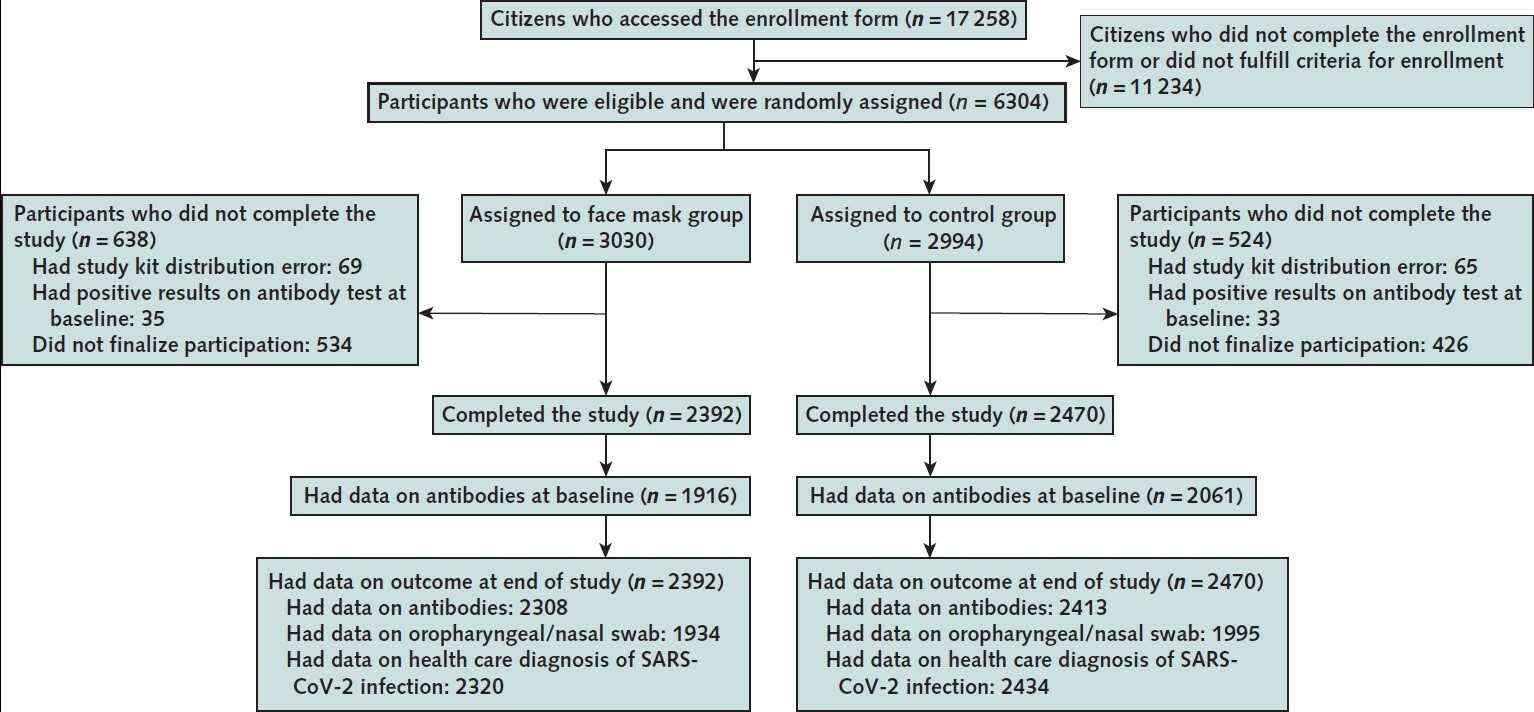
\includegraphics{fig/Bundgaard_Study_Flow.jpg}

\ldots{}

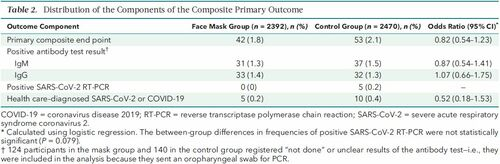
\includegraphics{fig/Bundgaard_Outcome_Components.jpg}

\emph{Taleb's Points:}

\begin{quote}
The Mask Group has 0/2392 PCR infections vs 5/2470 for the Control Group. Note that this is the only robust result and the authors did not test to see how nonrandom that can be. They missed on the strongest statistical signal. (One may also see 5 infections vs.~15 if, in addition, one accounts for clinically detected infections.)
\end{quote}

\begin{quote}
The rest, 42/2392 vs.~53/2470, are from antibody tests with a high error rate
which need to be incorporated via propagation of uncertainty-style methods
on the statistical significance of the results.
Intuitively a false positive rate with an expected ``true value'' \(p\)
is a random variable \(\rightarrow\) Binomial Distribution with STD \(\sqrt{n p (1-p)}\)
\end{quote}

\begin{quote}
False positives must be deducted in the computation of the odds ratio.
\end{quote}

\begin{quote}
\textbf{The central problem is that both p and the incidence of infection are in the tails!}
\end{quote}

\begin{quote}
As most infections happen at home, the study does not inform on masks in general --it uses wrong denominators for the computation of odds ratios (mixes conditional and unconditional risk). Worse, the study is not even applicable to derive information on masks vs.~no masks outside the house since during most of the study (April 3 to May 20, 2020), ``cafés and restaurants were closed ``, conditions too specific and during which the infection rates are severely reduced --tells us nothing about changes in indoor activity. (The study ended June 2, 2020). A study is supposed to isolate a source of risk; such source must be general to periods outside the study (unlike cardiology with unconditional effects).
\end{quote}

\begin{quote}
The study does not take into account the fact that masks might protect others. Clearly this is not cardiology but an interactive system.
\end{quote}

\begin{quote}
Statistical signals compound. One needs to input the entire shebang, not simple individual tests to assess the joint probability of an effect.
\end{quote}

\emph{Comment from Tom Wenseleers}
For the 5 vs 0 PCR positive result the p value you calculate is flawed. The correct way to do it would e.g.~be using a Firth logistic regression. Using R that would give you:

\begin{verbatim}
library(brglm)
summary(brglm(cbind(pcrpos, pcrneg) ~ treatment, family=binomial, data=data.frame(treatment=factor(c(“masks”,”nomasks”)),
pcrpos=c(0,5), pcrneg=c(2392,2470-5))))

2-sided p=0.11.
So that’s not significantly different.

Alternatively, you might use a Fisher’s exact test, which would give you :

fisher.test(cbind(c(0,2392),c(5,2470-5))):

2-sided p = 0.06.
Again, not significantly different.
\end{verbatim}

A Firth logistic regression would be more appropriate though, since we have a clear outcome variable here and we don't just want to test for an association in a 2×2 contingency table, as one would do using a Fisher's exact test. For details see Firth, D. (1993). Bias reduction of maximum likelihood estimates. Biometrika 80, 27--38. A regular logistic regression doesn't work here btw because of complete separation, \url{https://en.wikipedia.org/wiki/Separation_(statistics)} \url{https://stats.stackexchange.com/questions/11109/how-to-deal-with-perfect-separation-in-logistic-regression}. Going Bayesian would also be a solution, e.g.~using the bayesglm() or brms package, or one could use an L1 or L2 norm or elastic net penalized binomial GLM model, e.g.~using glmnet.

But the p value you calculate above is definitely not correct. Sometimes it helps to not try to reinvent the wheel.

The derivation of Fisher's exact test you can find in most Statistics 101 courses, see e.g.~\url{https://mathworld.wolfram.com/FishersExactTest.html}. For Firth's penalized logistic regression, see \url{https://medium.com/datadriveninvestor/firths-logistic-regression-classification-with-datasets-that-are-small-imbalanced-or-separated-49d7782a13f1} for a derivation. Or in Firth's original article: \url{https://www.jstor.org/stable/2336755?seq=1\#metadata_info_tab_contents}.

Technically, the problem with the way you calculated your p value above is that you use a one-sample binomial test, and assume there is no sampling uncertainty on the p=5/2470. Which is obviously not correct. So you need a two-sample binomial test instead, which you could get via a logistic regression. But since you have complete separation you then can't use a standard binomial GLM, and have to use e.g.~a Firth penalized logistic regression instead. Anyway, the details are in the links above.

You write ``The probability of having 0 realizations in 2392
if the mean is \(\frac{5}{2470}\) is 0.0078518, that is 1 in 127.
We can reexpress it in p values, which would be \textless.01''.
This statement is obviously not correct then.

And if you didn't do p values -- well, then your piece above is a little weak as a reply on how the authors should have done their hypothesis testing in a proper way, don't you think? If the 0 vs 5 PCR positive result is not statistically significant I don't see how you can make a sweeping statement like ``The Mask Group has 0/2392 PCR infections vs 5/2470 for the Control Group. Note that this is the only robust result and the authors did not test to see how nonrandom that can be. They missed on the strongest statistical signal.''. That ``strong statistical signal'' you mention turns out not be statistically significant at the p\textless0.05 level if you do your stats properly\ldots{}

Taleb:You are conflating p values and statistical significance.
Besides, I don't do P values. \url{https://arxiv.org/pdf/1603.07532.pdf}

you can also work with Bayes Factors if you like. Anything more formal than what you have above should do really\ldots{} But just working with a PMF of a binomial distribution, and ignoring the sampling error on the 5/2470 control group is not OK. And if you're worried about the accuracy of p values you could always still calculate 95\% confidence limits on them, right? Also not really what people would typically consider p-hacking\ldots{}

Your title may a bit of a misnomer then. And as I mentioned: if one is worried about the accuracy of your p values \& stochasticity on its estimated value, you can always calculate p-value prediction intervals, \url{https://royalsocietypublishing.org/doi/10.1098/rsbl.2019.0174}.

You are still ignoring the sampling uncertainty on the 0/2392. If you would like to go Monte Carlo you can use an exact-like logistic regression (\url{https://www.jstatsoft.org/article/view/v021i03/v21i03.pdf}). Using R, that gives me

For the 0 vs 5 PCR positive result:

\begin{verbatim}
library(elrm)
set.seed(1)
fit = elrm(pcrpos/n ~ treatment, ~ treatment,
r=2, iter=400000, burnIn=1000,
dataset=data.frame(treatment=factor(c(“masks”, “control”)), pcrpos=c(0, 5), n=c(2392, 2470)) )
fit$p.values # p value = 0.06, ie just about not significant at the 0.05 level
fit$p.values.se # standard error on p value = 0.0003 # this is very close to the 2-sided Fisher exact test p value
fisher.test(cbind(c(0,2392), c(5,2470-5))) # p value = 0.06

For the 0 vs 15 result:
set.seed(1)
fit = elrm(pcrpos/n ~ treatment, ~ treatment,
r=2, iter=400000, burnIn=1000,
dataset=data.frame(treatment=factor(c(“masks”, “control”)), pos=c(5, 15), n=c(2392, 2470)) )
fit$p.values # p value = 0.04 – this would be just about significant at the 0.05 level
fit$p.values.se # standard error on p value = 0.0003
\end{verbatim}

So some evidence for the opposite conclusions as what they have (especially for the 5 vs 15 result), but still not terribly strong.

Details of method are in \url{https://www.jstatsoft.org/article/view/v021i03/v21i03.pdf}.

I can see you don't like canned statistics. And you could recode these kinds of methods quite easily in Mathematica if you like, see here for a Fisher's exact test e.g.:
\url{https://mathematica.stackexchange.com/questions/41450/better-way-to-get-fisher-exact}.

But believe me -- also Sir Ronald Fisher will have thought long and hard about these kinds of problems. And he would have seen in seconds that what you do above is simply not correct. Quite big consensus on that if I read the various comments here by different people\ldots{}

I was testing the hypothesis of there being no difference in infection rate between both groups and so was doing 2-sided tests. Some have argued that masks could actually make things worse if not used properly. So not doing a directional test would seem most objective to me. But if you insist, then yes, you could use 1-tailed p values\ldots{} Then you would get 1-sided p values of 0.03 and 0.02 for the 0 vs 5 and 5 vs 15 sections of the data. Still deviates quite a bit from the p\textless0.01 that you first had.

In terms of double column joint distribution: then I think your code above should have e.g.~15/2470 and 5/2392 as your expectation of the Bernoulli distribution for vs 5 vs 15 comparison. But that would give problems for the 0/2392 outcome for the masks group in the 0 vs 5 comparison. As simulated Bernouilli trials with p=0 will be all zeros. Also, right now I don't see where that 2400 was coming from in your code. I get that you are doing a one-sided two-sample binomial test here via a MC approach. That's not the same than a Fisher exact test though.

\emph{Andreas:}
Weird, the last part of my comment above apparently got chopped up somehow. Ignore the CI calculations as they got messed up, but are trivial. Trying again with the text that got lost, containing my main point:

So the false positive-adjusted Odds Ratio is .71 {[}95\% CI .41, 1.21{]}, using the same model as the authors of the paper did. This can be compared to their reported OR = .82 {[}95\% CI .54, 1.23{]}.

Even with my quite conservative adjustment, the only robust finding claimed in the paper is not robust anymore -- the estimated risk reduction is no longer significantly lower than 50\%, according to the same standard logistic model used by the authors. Nor is it sig. larger than 0\%. The CI did not really improve over the unadjusted one (maybe this was obvious a priori, but not to me). Either way I think .71 is a better estimate than the .82 that was reported in the paper, based on Nassim's reasoning about the expected false positives. And .71 vs.~.82 might well have crossed the line for a mask policy to be seriously considered, by some policymaker who rejected .82 as too close to 1.

Sensitivity analysis of the FPR adjustment:
1\% FPR (Nassim's suggestion from the blog post) =\textgreater{} OR = .66 {[}95\% CI .36, 1.19{]}
.5\% FPR (lower estimate from the Bundgaard et al.~paper, based on a previous study) =\textgreater{} OR = .76 {[}95\% CI .47, 1.22{]}

\emph{Tom}

I do agree with all the shortcomings of this study in general though. It certainly was massively underpowered.

\emph{Other comments:}

\href{https://pubmed.ncbi.nlm.nih.gov/33205991/}{Bundgaard (2020) Effectiveness of Adding Mask}
\href{https://www.acpjournals.org/doi/10.7326/M20-6817}{Same in Annals}

\href{pdf/Bundgaard_2020_Mask_Effectiveness_ref_Taleb.pdf}{(pdf)}

\href{https://fooledbyrandomnessdotcom.wordpress.com/2020/11/25/hypothesis-testing-in-the-presence-of-false-positives-the-flaws-in-the-danish-mask-study/}{Taleb Review of Bundgaard}

\href{https://medium.com/incerto/the-masks-masquerade-7de897b517b7}{Taleb Medium}

\href{https://www.ncbi.nlm.nih.gov/pmc/articles/PMC2938757/}{Odd's Ratio Explained (NIH)}

\emph{Composite Endpoints:}

Composite endpoints in clinical trials are composed of primary endpoints that contain two or more distinct component endpoints. The purported benefits include increased statistical efficiency, decrease in sample-size requirements, shorter trial duration, and decreased cost. However, the purported benefits must be diligently weighed against the inherent challenges in interpretation. Furthermore, the larger the gradient in importance, frequency, or results between the component endpoints, the less informative the composite endpoint becomes, thereby decreasing its utility for medical-decision making.

{[}Composite Endpoints (NIH){]} (\url{https://www.ncbi.nlm.nih.gov/pmc/articles/PMC6040910/})

\href{https://en.wikipedia.org/wiki/Separation_(statistics)}{Separation (Wikipedia)}

\href{https://www.ncbi.nlm.nih.gov/pmc/articles/PMC5654877/}{Intention to treat vs Per Protocol}

\hypertarget{fat-tails}{%
\chapter{Fat Tails}\label{fat-tails}}

\begin{verbatim}
Extremes      
    Catastrophe Principle  
Statistical Consequences of Fat Tails  
Power Law Distributions  
    Pareto Distribution  
Pandemic Risk Management
\end{verbatim}

Fat tails and ergodicity tell you the same thing.
You're not going to find the truth through evidence.
You find it through time.
Academia and science currently are missing this point.
Popper. Falsification works in theory but gets hijacked by money and politics in practice.
(Portesi)

Science uses statistics \&, as per Popper, doesn't really ``accept'',
just fails to reject at some significance.
It's fundamentally disconfirmatory.
Stat. ``evidence'' is inherently probabilistic and
cannot be ``degenerate'' (i.e.~provide certainties).
(Taleb)

\hypertarget{extremes}{%
\section{Extremes}\label{extremes}}

The field of Extreme Value Theory focuses on tail properties,
not the mean or statistical inference.

It is vastly more effective
to focus on being insulated from the harm of random events
than try to figure them out in the required details
(the inferential errors under fat tails are huge).
So it is more solid, much wiser, more ethical, and more effective to focus on
detection heuristics and policies rather than fabricate statistical properties.

\hypertarget{catastrophe-principle}{%
\subsection{Catastrophe Principle}\label{catastrophe-principle}}

\emph{Memo Taleb (DarwinCollege):}

Where a Pareto distribution
prevails (among many), and randomly select two people with
combined wealth of £36 million. The most likely combination
is not £18 million and £18 million. It is approximately
£35,999,000 and £1,000. This highlights the crisp distinction
between the two domains; for the class of subexponential
distributions, \emph{ruin is more likely to come from a single extreme
event than from a series of bad episodes}. This logic underpins
classical risk theory as outlined by Lundberg early in the 20 th
Century and formalized by Cramer, but forgotten by
economists in recent times. This indicates that insurance can
only work in Medocristan; you should never write an uncapped
insurance contract if there is a risk of catastrophe. The point
is called the catastrophe principle.

Cramer showed insurance could not work outside
what he called the Cramer condition, which excludes possible
ruin from single shocks.

With fat tail distributions, extreme events
away from the centre of the distribution play a very large
role. Black swans are not more frequent, they are more
consequential. The fattest tail distribution has just one very
large extreme deviation, rather than many departures form the
norm.

There are three types of fat tails based on mathematical properties.

First there are entry level fat tails.
This is any distribution with fatter tails than the Gaussian
i.e.~with more observations within one sigma and with
kurtosis (a function of the fourth central moment) higher than three.

Second, there are subexponential distributions.

\emph{LogNormal:}

The subexponential class includes the lognormal, which is one
of the strangest things on earth because sometimes it cheats
and moves up to the top of the diagram. At low variance, it is
thin-tailed, at high variance, it behaves like the very fat tailed.
in-tailed, at high variance, it behaves like the very fat tailed.

Membership in the subexponential class satisfies the Cramer
condition of possibility of insurance (losses are more likely to
come from many events than a single one)
Technically it means that the expectation of
the exponential of the random variable exists.

Third, what is called by a variety of names, the power law, or slowly
varying class, or ``Pareto tails'' class correspond to real fat tails.

The traditional statisticians approach to fat tails has been
to assume a different distribution but keep doing business as
usual, using same metrics, tests, and statements of significance.
But this is not how it really works and they fall into logical
inconsistencies.

Once we are outsaide the zone for which statistical techniques were designed,
things no longer work as planned.
Here are some consequences

\begin{enumerate}
\def\labelenumi{\arabic{enumi})}
\item
  The law of large numbers, when it works, works too slowly in the real
  world (this is more shocking than you think as it cancels most statistical estimators)
\item
  The mean of the distribution will not correspond to the sample mean.\\
  In fact, there is no fat tailed distribution in which the mean can be properly
  estimated directly from the sample mean,
  unless we have orders of magnitude more data than we do
\item
  Standard deviations and variance are not useable. They fail out of sample.
\item
  Beta, Sharpe Ratio and other common financial metrics
  are uninformative.
\item
  Robust statistics is not robust at all.
\item
  The so-called ``empirical distribution'' is not empirical
  (as it misrepresents the expected payoffs in the tails).
\item
  Linear regression doesn't work.
\item
  Maximum likelihood methods work for parameters
  (good news). We can have plug in estimators in some
  situations.
\item
  The gap between dis-confirmatory and confirmatory
  empiricism is wider than in situations covered by common
  statistics i.e.~difference between absence of evidence and
  evidence of absence becomes larger.
\item
  Principal component analysis is likely to produce false
  factors.
\item
  Methods of moments fail to work. Higher moments are
  uninformative or do not exist.
\item
  There is no such thing as a typical large deviation:
  conditional on having a large move, such move is not
  defined.
\item
  The Gini coefficient ceases to be additive. It becomes
  super-additive. The Gini gives an illusion of large con-
  centrations of wealth. (In other words, inequality in a
  continent, say Europe, can be higher than the average
  inequality of its members).
\end{enumerate}

While it takes 30 observations in the Gaussian to stabilize
the mean up to a given level,
it takes \(10^{11}\) observations in the Pareto to bring the sample error down
by the same amount (assuming the mean exists).
You cannot make claims about the stability of the sample
mean with a fat tailed distribution. There are other ways to do
this, but not from observations on the sample mean.

We have known at least since Sextus Empiricus that we
cannot rule out degeneracy but there are situations in which
we can rule out non-degeneracy. If I see a distribution that
has no randomness, I cannot say it is not random. That is,
we cannot say there are no black swans. Let us now add
one observation. I can now see it is random, and I can
rule out degeneracy. I can say it is not not random. On the
right hand side we have seen a black swan, therefore the
statement that there are no black swans is wrong. This is the
negative empiricism that underpins Western science. As we
gather information, we can rule things out.
If we see a 20 sigma event, we can rule out that the
distribution is thin-tailed.

\emph{Pareto - Scalability}

The intuition behind the Pareto Law. It is simply defined as:
say X is a random variable.
For x sufficently large, the probability of exceeding 2x divided by the
probability of exceeding x is no different from the probability
of exceeding 4x divided by the probability of exceeding 2x,
and so forth.

So if we have a Pareto (or Pareto-style) distribution, the ratio
of people with £16 million compared to £8 million is the same
as the ratio of people with £2 million and £1 million. There
is a constant inequality.

This distribution has no characteristic
scale which makes it very easy to understand. Although this
distribution often has no mean and no standard deviation we
still understand it. But because it has no mean we have to
ditch the statistical textbooks and do something more solid,
more rigorous.

A Pareto distribution has no higher moments: moments
either do not exist or become statistically more and more
unstable.

In 2009 I took 55 years of data and
looked at how much of the kurtosis (a function of the fourth
moment) came from the largest observation. For
a Gaussian the maximum contribution over the same time span
should be around .008 ± .0028. For the S\&P 500 it was about
80 per cent. This tells us that we dont know anything about
kurtosis. Its sample error is huge; or it may not exist so the
measurement is heavily sample dependent. If we dont know
anything about the fourth moment, we know nothing about the
stability of the second moment. It means we are not in a class
of distribution that allows us to work with the variance, even
if it exists. This is finance.

We cannot use standard statistical methods with financial data.

Financial data, debunks all the college textbooks we are currently using
Econometrics that deals with squares goes out of the window.
The variance of the squares is analogous to the fourth moment.
The variance of the squares is analogous to the fourth moment.
We do not know the variance. But we can work very easily
with Pareto distributions. They give us less information, but
nevertheless, it is more rigorous if the data are uncapped or if
there are any open variables.

Principal component analysis is a dimension
reduction method for big data and it works beautifully with
thin tails. But if there is not enough data there is an illusion
of a structure. As we increase the data (the n variables),
the structure becomes flat.

\emph{Lessons:}

Once we know something is fat-tailed, we can use heuristics to see
how an exposure there reacts to random events: how much
is a given unit harmed by them. It is vastly more effective
to focus on being insulated from the harm of random events
than try to figure them out in the required details (as we saw
the inferential errors under fat tails are huge). So it is more
solid, much wiser, more ethical, and more effective to focus on
detection heuristics and policies rather than fabricate statistical
properties.

The beautiful thing we discovered is that everything that is
fragile has to present a concave exposure similar --if not
identical --to the payoff of a short option, that is, a negative
exposure to volatility. It is nonlinear, necessarily. It has to
have harm that accelerates with intensity, up to the point of
breaking. If I jump 10m I am harmed more than 10 times than
if I jump one metre. That is a necessary property of fragility.

We just need to look at acceleration in the tails. We have built
effective stress testing heuristics based on such an option-like
property.

In the real world we want simple things that work;
we want to impress our accountant and not our peers. (My
argument in the latest instalment of the Incerto, Skin in the
Game is that systems judged by peers and not evolution rot
from overcomplication). To survive we need to have clear
techniques that map to our procedural intuitions.

The new focus is on how to detect and measure convexity and concavity.
This is much, much simpler than probability.

\href{/pdf/Taleb_2017_Extremes_DarwinCollege.pdf}{Taleb (2017) Darwin Colleges(pdf)}

\hypertarget{statistical-consequences-of-fat-tails}{%
\section{Statistical Consequences of Fat Tails}\label{statistical-consequences-of-fat-tails}}

\begin{quote}
Conventional statistics fail to cover fat tails;
physicists who use power laws do not usually produce statistical estimators.
\end{quote}

\href{https://www.fooledbyrandomness.com/FatTails.html}{Taleb's Research Site}

\begin{quote}
Take nothing for granted - \emph{It is what it is.}
Another 300 years of data is required to test a statistical hypothesis.
A dataset has no variance.
A distribution's standard deviation will not converge in a lifetime's worth of data.
\end{quote}

Fat tailed random variables challenge our conceptions of mean and standard deviation.
Linear regression also breaks under fat tails.
The convincing case is made that power law distributions should be the default
for modeling data rather than the thin-tailed Normal distribution.

Any distribution with more density in the tails than the Normal distribution
is said to have thick tails.
This corresponds to raw kurtosis \textgreater{} 3.
The tail density needs to decay slower than Normal, \(\frac{-x^2}{e^{2\sigma^2}}\).

Fat tailed distributions are the thickest tailed distributions.
The power law is an example of this -
they're the distributions with so much additional density in their tails
that moments \(E[X^p]\) are no longer finite.

\emph{Zweig}

To be insurable, events must be non-subexponential i.e.~the probability of exceeding some threshold must be due to a series of small events rather than a single large event. The Cramer condition must also be met (exponential moments of the rv must exist). Normally distributed events meet these conditions, but not thick tailed events. In the former case, exceeding some threshold is more likely to come from a series of events (increasingly so as you move into the tails due to exponential decay of tail probabilities)\ldots hence focus on reducing frequency of events. In the latter case, exceeding some threshold is more likely to come from a single event, so focus must be on reducing impact.

The Lucretius fallacy is when one assumes the worst event experienced in the past is the worst event that can happen in the future. Because an empirical distribution is necessarily censured by x\_min and x\_max, the empirical distribution is not empirical. Beyond the observed max, there is a hidden portion of the distribution not shown in past samples whose moments are unknown (and do not converge via the Glivenko-Cantelli theorem). This is a problem for Kolmogorov-Smirnoff tests. It is better to use MLE to get the `excess' or `shadow' mean (the mean beyond the sample max). Assuming you can estimate the tail exponent, this approach works better for out-of-sample inference than use of the sample mean (biased under thick tails). The lower the tail exponent and smaller the sample, the more the tail is hidden.

The precautionary principle is necessary for higher order units (ecosystem, humanity, etc.) that do not ``renew'' the way lower order units do (individual people, animals, goods, etc.). With repeated exposure to a low-probability event, its probability of occurrence will approach 1 over time. If one's exposure f(x) has an absorbing barrier, they must focus on time probability (path dependence) rather than ensemble probability (path independence). Since financial asset prices, particularly equities, are non-ergodic (time average \textless\textgreater{} ensemble average due to fat tails), one is not guaranteed the return of the market unconditionally. Hence the myopic loss aversion explanation (increased sensitivity to losses and less willingness to accept risk the more often you check performance) of the equity risk premium puzzle falls apart. Risks accumulate for individuals, making it rational to be loss averse and avoid tail risks.

\href{https://www.amazon.com/review/RMD3OUG0WQWWY/ref=cm_cr_srp_d_rdp_perm?ie=UTF8\&ASIN=1544508050}{Zweig: Suimmary of Talebs `Fat Tails'}

\hypertarget{power-law-distributions}{%
\subsection{Power Law Distributions}\label{power-law-distributions}}

\hypertarget{pareto-distribution}{%
\subsubsection{Pareto Distribution}\label{pareto-distribution}}

Pareto discovered that 20\% percent of taxpayers had 80\% of the income across countries in Europe.
One parameter of the Pareto power law distribution is α, which is known as the \emph{tail index}.
Pareto's 80-20 example corresponds to α = 1.16.
The tail index describes the behavior of density decay in the tail, as its name implies.

The strange thing about power law distributions is that, depending on the tail index α,
some of its moments may not exist or be infinite.
There is no finite mean if α \textless{} 1,
and there is no finite variance if α \textless{} 2.
The same applies for skewness at α \textless{} 3 and kurtosis when α \textless{} 4, and so on.
The tails get thicker as α gets smaller.

Pseudo-convergence: A tail index less than 2 doesn't mean that we can't compute the sample variance of dataset. Rather, betting on the stability of the variance is unwise because this sample variance will never converge, and can in fact ``spike'' at any time. Furthermore, if the 4th moment (kurtosis) doesn't exist, this may imply unbearably slow convergence of the 2nd moment (variance).

The Central Limit Theorem, which is typically very useful for sums and averages, requires a finite variance, so tail indices α \textless{} 2 do not obey. The assumption for the analytic Black-Scholes-Merton price for a financial option - that the random walk sum of movements converges to the Normal distribution - is also violated, so that breaks too. If the tail index is slightly over 2, it will converge to the Normal in the limit, but very slowly.

\emph{Tail events} - the unlikely events of the atypically large magnitude - are the most indicative of the tail behavior. But these tail events are rare. Without a deep understanding of the underlying process which has generated these samples, it can be tough to rule out that the data was generated by a power law. In this sense, we might consider that ``most'' processes are fat tailed by default - or, we should at least assume they are until we have enough quantitative or qualitative data to prove otherwise.

\href{https://gelman.me/scoft.html}{Review of Taleb (Gelman)}

\hypertarget{lindy-effect}{%
\section{Lindy Effect}\label{lindy-effect}}

\emph{Increasing lifetime expections}

\begin{quote}
If a book has been in print for forty years, I can expect it to be in print for another forty years. But, and that is the main difference, if it survives another decade, then it will be expected to be in print another fifty years. This, simply, as a rule, tells you why things that have been around for a long time are not ``aging'' like persons, but ``aging'' in reverse. Every year that passes without extinction doubles the additional life expectancy. This is an indicator of some robustness. The robustness of an item is proportional to its life! (\emph{Taleb})
\end{quote}

\emph{Pareto Lindy}

Lifetimes following the Pareto distribution (a power-law distribution) demonstrate the Lindy effect.

With the parameter \(α = 2\), conditional on reaching an age of \(x > x_{min}\),
the expected future lifetime is also \(x\).

Initially the expected lifetime is \(2 x_{min}\) but if that point is reached
then the expected future lifetime is also \(2 x_{min}\);
if that point is reached making the total lifetime so far \(4 x_{min}\)
then the expected future lifetime is \(4 x_{min}\); and so on.

More generally with proportionality rather than equality,
given \(m > 0\) and using the parameter \(\alpha = \frac {m}{m-1}\)
in the Pareto distribution, conditional on reaching any age of \(x > x_{min}\),
the expected future lifetime is \(( m − 1 ) x\).

Example: for \(α = 2\) or \(m = 2\) the expected future lifetime is \(x\) .

The Lindy effect is connected to Pareto's Law, to Zipf's Law, and to socioeconomic inequality.

\href{https://en.wikipedia.org/wiki/Lindy_effect}{Wikipedia: Lindy Effect}

Current age is the only piece of information we know at time 0.
In the absence of all information except for current age,
the best estimator for future life expectancy is the current age.

In real life, however, there is usually far more information you can incorporate.
The Lindy Effect is thus a trivial heuristics,
the usefulness of which decreases as if you acquire additional relevant information.

\href{https://cryptowords.github.io/the-statistical-fallacy-behind-the-lindy-effect}{Wang: Lindy Fallacy}

\href{https://towardsdatascience.com/a-statistical-rule-to-optimize-your-life-the-lindys-effect-96d2c75b080d}{Doan: Lindy Simulation}

\href{https://alevchuk.medium.com/statistical-testing-of-the-lindy-effect-with-real-data-4f55a5a9a2f0}{Levchuk: Testing Lindy}

\hypertarget{superspreaders}{%
\section{Superspreaders}\label{superspreaders}}

\emph{Wong}

Superspreading has been recognized as an important phenomenon arising from heterogeneity in individual disease transmission patterns (1). The role of superspreading as a significant source of disease transmission has been appreciated in outbreaks of measles, influenza, rubella, smallpox, Ebola, monkeypox, SARS, and SARS-CoV-2 (1, 2). A basic definition of an nth-percentile superspreading event (SSE) has been proposed to be any infected individual who infects more people than does the nth-percentile of other infected individuals (1). Hence, if the number of secondary cases is randomly distributed, then for large n, SSEs can be viewed as right-tail events. A natural language for understanding the tail events of random distributions is extreme value theory, which has been applied to contexts as diverse as insurance (3) and contagious diseases (4). Here, we apply extreme value theory to empirical data on superspreading in order to gain insight into this critical phenomenon impacting the current COVID-19 pandemic.

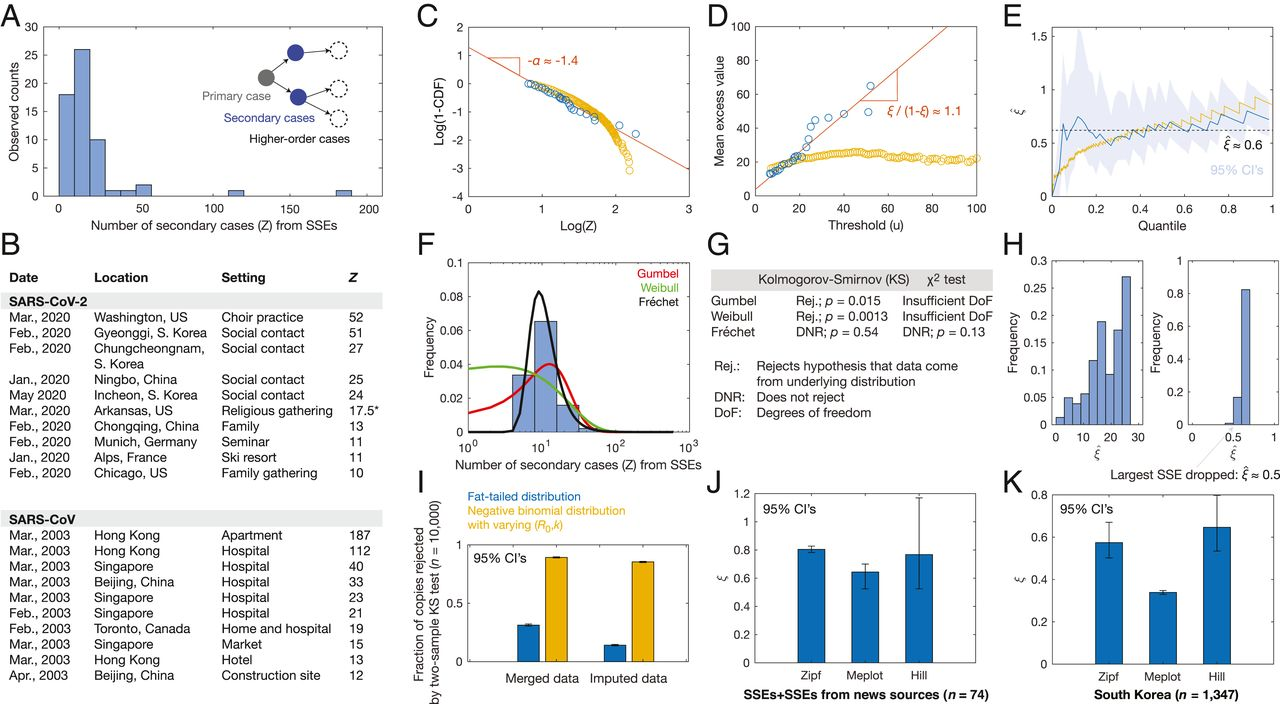
\includegraphics{fig/Wong_Superspreader.jpg}

Figure: SARS-CoV and SARS-CoV-2 SSEs correspond to fat tails.
(A) Histogram of Z for 60 SSEs.
(B) Subsample of 20 diverse SARS-CoV and SARS-CoV-2 SSEs. *See Dataset S1 for details.
(C) Zipf plots of SSEs (blue) and 10,000 samples of a negative binomial distribution
with parameters (R0,k) = (3,0.1), conditioned on Z \textgreater{} 6 (yellow).
(D) Meplots corresponding to C.
(E) Plots of \(\hat{ξ}\), the Hill estimator for ξ, for the samples in C.
(F) Different extreme value distribution fits to the distribution of SSEs.
(G) One-sample Kolmogorov--Smirnov and \(χ^{2}\) goodness-of-fit test results for the fits in F.
(H) Robustness of results, accounting for noise (Left) and incomplete data (Right).
(I) Inconsistency of the maxima of 10,000 samples of a negative binomial distribution (yellow)
with the SSEs in A, accounting for variability in (R0,k) and data merging and imputation,
in contrast to the maxima of 30 samples from a fat-tailed (Fréchet) distribution (blue)
with tail parameter α = 1.7 and mean R0 = 3.
The numbers of samples in each case were determined so that
the sample mean of maxima is equal to the sample mean from A.
(J--K) Generality of inferred \(ξ\) to 14 additional SSEs from news sources
(J) and a dataset of 1,347 secondary cases arising from 5,165 primary cases in South Korea
(K).

The Zipf plot shown in Fig.1C is a log-log plot of the survival function against the number
of secondary cases, and the linearly decreasing behavior it shows
suggests a power-law scaling of the form \$Pr(Z\textgreater t)\textasciitilde t\^{}\{α\} for large t.
The value of the power-law coefficient, \(α≈1.45\) (95\% CI: {[}1.38,1.51{]}), is greater than 1.
Equivalently, this observation indicates that the tails of \(Z\) ---as quantified by the threshold
exceedance values \({Z_{i–u} | Z_{i} ≥u}\) ---can be described by the generalized Pareto distribution,
withcorresponding tail index \(ξ=1/α ≈ 0.7\) (95\% CI: {[}0.62,0.76{]}).
That \(ξ≤1\) is significant,
since all moments higher than \(1/ξ\) diverge for a generalized Pareto distribution.
The Zipf plot can be complemented by computing
the mean excess function of \(Z\), \(e(u) = E(Z–u | Z≥u)\), which
for a generalized Pareto distribution is linear in \(u\) with slope \(ξ/(1–ξ)\).
Hence, checking for linearity in a plot of \(u\) against \(e(u) — a\) mean excess plot --- above some threshold u allows one to verify the existence
of fat tails. We observed in a meplot that for u\textgreater10, e(u) indeed increases approximately linearly with a
slope of \textasciitilde1.11 (Fig.1D; 95\% CI: {[}1.02,1.20{]}; adjusted \(R^{2}\) : 0.91),
suggesting a value of \(ξ≈0.5\), which is
qualitatively consistent with the Zipf plot of Fig.1C

The Hill estimator of the tail index \(ξ\) is

\[\hat{ξ}(k) = \frac{1}{k} \sum_{i=1}^{k} log \frac{Z_{i,n}}{Z_{k,n}}\]

where 2≤k≤n and Z n,n ≤Z n-1,n ≤\ldots≤Z 1,n are order statistics of the sample \{Z i \}. Plotting \(ξ\) against \(k\), we find
that the value of \(ξ ≈0.6\) (95\% CI: {[}0.4,1.0{]}) observed for a broad range of \(k\) is similar to the estimates
above (Fig.1E).
We found similar values of \(ξ\) for two other estimators, the Pickands and
Dekkers-Einmahl-de Haan estimators.
A negative binomial distribution of Z, with its exponential tail, would have
predicted the distribution of SSEs to be Gumbel-like if each SSE were indeed
a maximum of samples of \(Z\).
This assertion can be proven by verifying the conditions

\[\underset{n\to \infty}{\lim} \frac{\sum_{n}^{\infty} P_{j}}{\sum_{n+1}^{\infty} P_{j}} = const\]

\[\underset{n\to \infty}{\lim} \sum_{n+2}^{\infty} \frac{P_{j}}{P_{n+1}}-\sum_{n+1}^{\infty}\frac{P_{j}}{P_{n}}= 0\]

where \(P_{j} =Pr(Z=j)\), sufficient for any discrete distribution to lie in a Gumbel-like domain of attraction.
These considerations provide additional evidence suggesting that Z is not negative binomial.

\href{coronavirus\%20superspreading\%20is\%20fat-tailed}{Wong (2021) Coronavirus superspreading is fat-tailed (PNAS)}
\href{pdf/Wong_2021_Corona_Superspreader_Fat-tailed.pdf}{(pdf)}
\href{pdf/Wong_2021_Corona_Superspreader_Fat-tailed_SM.pdf}{(pdf SM)}

\hypertarget{vaccine}{%
\chapter{Vaccine}\label{vaccine}}

\emph{Madhi}

A multicenter, double-blind, randomized, controlled trial to assess the safety and efficacy of the ChAdOx1 nCoV-19 vaccine (AZD1222) in people not infected with the human immunodeficiency virus (HIV) in South Africa. Participants 18 to less than 65 years of age were assigned in a 1:1 ratio to receive two doses of vaccine containing 5×1010 viral particles or placebo (0.9\% sodium chloride solution) 21 to 35 days apart. Serum samples obtained from 25 participants after the second dose were tested by pseudovirus and live-virus neutralization assays against the original D614G virus and the B.1.351 variant. The primary end points were safety and efficacy of the vaccine against laboratory-confirmed symptomatic coronavirus 2019 illness (Covid-19) more than 14 days after the second dose.

Between June 24 and November 9, 2020, we enrolled 2026 HIV-negative adults (median age, 30 years); 1010 and 1011 participants received at least one dose of placebo or vaccine, respectively. Both the pseudovirus and the live-virus neutralization assays showed greater resistance to the B.1.351 variant in serum samples obtained from vaccine recipients than in samples from placebo recipients. In the primary end-point analysis, mild-to-moderate Covid-19 developed in 23 of 717 placebo recipients (3.2\%) and in 19 of 750 vaccine recipients (2.5\%), for an efficacy of 21.9\% (95\% confidence interval {[}CI{]}, −49.9 to 59.8). Among the 42 participants with Covid-19, 39 cases (92.9\%) were caused by the B.1.351 variant; vaccine efficacy against this variant, analyzed as a secondary end point, was 10.4\% (95\% CI, −76.8 to 54.8). The incidence of serious adverse events was balanced between the vaccine and placebo groups.

The primary efficacy analysis was end-point--driven for the composite of mild, moderate, or severe Covid-19 and required 42 cases to detect a vaccine efficacy of at least 60\% (with a lower bound of 0\% for the 95\% confidence interval), with 80\% power. Vaccine efficacy was calculated as 1 minus the relative risk, and 95\% confidence intervals calculated with the Clopper--Pearson exact method are reported. Only participants in the per-protocol population (all participants who received two doses of vaccine or placebo and were grouped according to the injection they received, regardless of their planned group assignment) who were seronegative for SARS-CoV-2 at enrollment were included in the primary efficacy analysis. A sensitivity analysis was conducted that included seronegative participants in the modified intention-to-treat population (all participants who received two doses and were grouped by their planned assignment, irrespective of the injection they received). Confidence intervals reported in this article have not been adjusted for multiple comparisons.

Conclusions

A two-dose regimen of the ChAdOx1 nCoV-19 vaccine did not show protection against mild-to-moderate Covid-19 due to the B.1.351 variant.

\href{https://www.nejm.org/doi/10.1056/NEJMoa2102214\#.YFJIkr3ju7k.twitter}{Madhi (2021) Efficacy Covid Vaccine}

\hypertarget{inequality}{%
\chapter{Inequality}\label{inequality}}

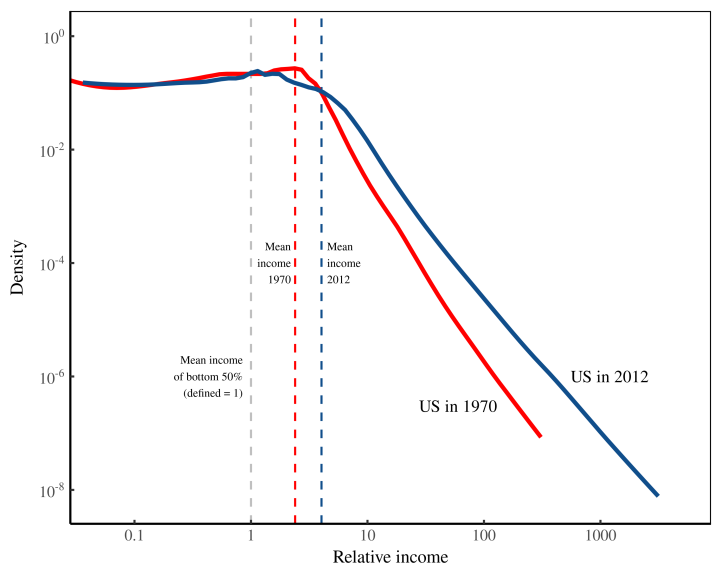
\includegraphics[width=5in,height=3.75in]{fig/fix_inequality.png}

\emph{Figure: How the US distribution of income has changed since 1970.
Probability density of US income in 1970 and 2012.
Normalized incomes so that the average income of the bottom half of Americans equals 1.
Note the log scales on both axes.}
Source \href{https://economicsfromthetopdown.com/2021/02/26/radically-progressive-degrowth-reducing-resource-use-by-eliminating-inequality/}{Blair Fix}

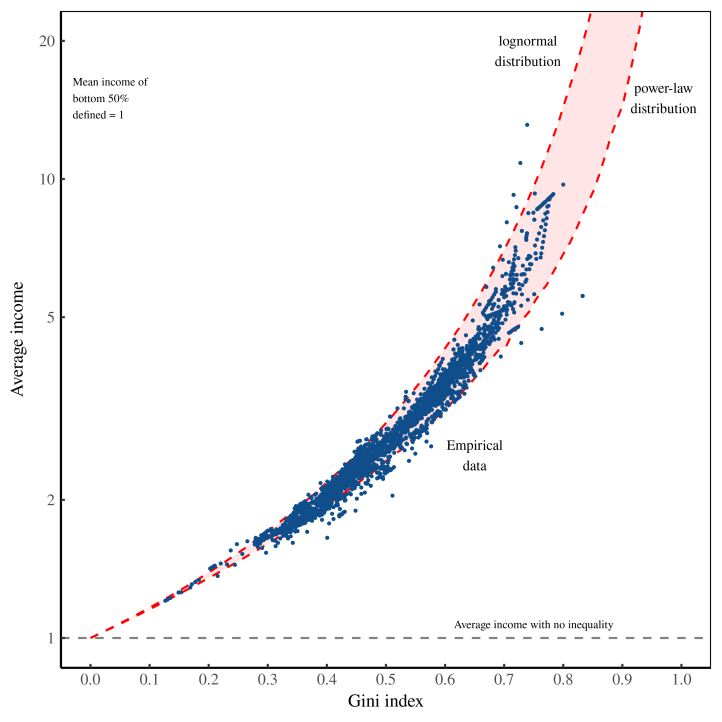
\includegraphics[width=5in,height=3.75in]{fig/fix_inequality_model.png}

Figure: Modeling radically progressive degrowth.
The horizontal axis shows income inequality (within countries), measured using the Gini index.
Blue points are empirical data.
The vertical axis shows average income (in a country),
defined so that the mean income of the bottom-half of earners equals 1.
The dashed red lines show the trend produced by ramping up inequality
in a lognormal distribution (left) and power-law distribution (right).
Source \href{https://economicsfromthetopdown.com/2021/02/26/radically-progressive-degrowth-reducing-resource-use-by-eliminating-inequality/}{Blair Fix}

\begin{itemize}
\tightlist
\item
  Abstract Blair Fix:*
\end{itemize}

What explains the power-law distribution of top incomes? This paper tests the
hypothesis that it is firm hierarchy that creates the power-law income distribution tail.
Using the available case-study evidence on firm hierarchy, I create the
first large-scale simulation of the hierarchical structure of the US private sector.
Although not tuned to do so, this model reproduces the power-law scaling of
top US incomes. I show that this is purely an effect of firm hierarchy. This raises
the possibility that the ubiquity of power-law income distribution tails is due to
the ubiquity of hierarchical organization in human societies.

\href{https://osf.io/u95dk/}{Blair Fix (2018) Hierarchy Power Law Income Distribution}
\href{pdf/Blair_Fix_2018_Hierarchy_Power_law.pdf}{(pdf)}

\hypertarget{autocorrelation}{%
\chapter{Autocorrelation}\label{autocorrelation}}

\emph{Fix}

Autocorrelation occurs when you correlate a variable with itself. For instance, if I measure the height of 10 people, I'll find that each person's height correlates perfectly with itself. If this sounds like circular reasoning, that's because it is. Autocorrelation is the statistical equivalent of stating that 5 = 5.

When framed this way, the idea of autocorrelation sounds absurd. No competent scientist would correlate a variable with itself. And that's true for the pure form of autocorrelation. But what if a variable gets mixed into both sides of an equation, where it is forgotten? In that cause, autocorrelation is more difficult to spot.

We define a variable called z, which is correlated strongly with x. The problem is that z happens to be the sum x + y. So we are correlating x with itself. The variable y adds statistical noise.

That's how autocorrelation happens --- forgetting that you've got the same variable on both sides of a correlation.

\href{https://economicsfromthetopdown.com/2022/04/08/the-dunning-kruger-effect-is-autocorrelation/}{Fix: The Dunning-Kruger Effect is Autocorrelation}

\hypertarget{dunning-kruger-is-autocorrelation}{%
\section{Dunning-Kruger is Autocorrelation}\label{dunning-kruger-is-autocorrelation}}

\emph{Fix}

Have you heard of the `Dunning-Kruger effect'? It's the (apparent) tendency for unskilled people to overestimate their competence. Discovered in 1999 by psychologists Justin Kruger and David Dunning, the effect has since become famous.

And you can see why.

It's the kind of idea that is too juicy to not be true. Everyone `knows' that idiots tend to be unaware of their own idiocy. Or as John Cleese puts it:

\begin{verbatim}
If you’re very very stupid, how can you possibly realize that you’re very very stupid? 
\end{verbatim}

Of course, psychologists have been careful to make sure that the evidence replicates. But sure enough, every time you look for it, the Dunning-Kruger effect leaps out of the data. So it would seem that everything's on sound footing.

Except there's a problem.

The Dunning-Kruger effect also emerges from data in which it shouldn't. For instance, if you carefully craft random data so that it does not contain a Dunning-Kruger effect, you will still find the effect. The reason turns out to be embarrassingly simple: the Dunning-Kruger effect has nothing to do with human psychology.1 It is a statistical artifact --- a stunning example of autocorrelation.

In 1999, Dunning and Kruger reported the results of a simple experiment. They got a bunch of people to complete a skills test. (Actually, Dunning and Kruger used several tests, but that's irrelevant for my discussion.) Then they asked each person to assess their own ability. What Dunning and Kruger (thought they) found was that the people who did poorly on the skills test also tended to overestimate their ability. That's the `Dunning-Kruger effect'.

To interpret the Dunning-Kruger chart, we (implicitly) look at the difference between the two curves. That corresponds taking `perceived ability' and subtracting from it `actual test score'. In my notation, that difference is y -- x (indicated by the double-headed arrow). When we judge this difference as a function of the horizontal axis, we are implicitly comparing y -- x to x. Since x is on both sides of the comparison, the result will be an autocorrelation.

We're comparing x with the negative version of itself. That is textbook autocorrelation. It means that we can throw random numbers into x and y --- numbers which could not possibly contain the Dunning-Kruger effect --- and yet out the other end, the effect will still emerge.

What's interesting is how long it took for researchers to realize the flaw in Dunning and Kruger's analysis. Dunning and Kruger published their results in 1999. But it took until 2016 for the mistake to be fully understood. To my knowledge, Edward Nuhfer and colleagues were the first to exhaustively debunk the Dunning-Kruger effect. (See their joint papers in \href{https://digitalcommons.usf.edu/cgi/viewcontent.cgi?article=1188\&context=numeracy}{2016} and \href{https://digitalcommons.usf.edu/cgi/viewcontent.cgi?article=1215\&context=numeracy}{2017}.) In 2020, Gilles Gignac and Marcin Zajenkowski published a similar \href{https://www.gwern.net/docs/iq/2020-gignac.pdf}{critique}.

The problem with the Dunning-Kruger chart is that it violates a fundamental principle in statistics. If you're going to correlate two sets of data, they must be measured independently.

What's important here is that people's `skill' is measured independently from their test performance and self assessment.

Mistakes happen. So in that sense, we should not fault Dunning and Kruger for having erred. However, there is a delightful irony to the circumstances of their blunder. Here are two Ivy League professors7 arguing that unskilled people have a `dual burdon': not only are unskilled people `incompetent' \ldots{} they are unaware of their own incompetence.

The irony is that the situation is actually reversed. In their seminal paper, Dunning and Kruger are the ones broadcasting their (statistical) incompetence by conflating autocorrelation for a psychological effect. In this light, the paper's title may still be appropriate. It's just that it was the authors (not the test subjects) who were `unskilled and unaware of it'.

\href{https://economicsfromthetopdown.com/2022/04/08/the-dunning-kruger-effect-is-autocorrelation/}{Fix: The Dunning-Kruger Effect is Autocorrelation}

\hypertarget{causation}{%
\chapter{Causation}\label{causation}}

\emph{Altman Abstract}

Correlation implies association, but not causation.
Conversely, causation implies association, but not correlation.

Associations can arise between variables in the presence (i.e., X causes Y) and
absence (i.e., they have a common cause) of a causal relationship

In everyday language, dependence, association and correlation are used interchangeably. Technically, however, association is synonymous with dependence and is different from correlation

\href{https://www.nature.com/articles/nmeth.3587}{Altman (2015) Association Correlation Causation}
\href{pdf/Altman_2015_Association_Correlation_and_Causation.pdf}{(pdf)}

\hypertarget{liang-causality}{%
\section{Liang Causality}\label{liang-causality}}

\textbf{Information Flow-Based Causality}

\emph{Liang (2016) Abstract}

Information flow or information transfer the widely applicable
general physics notion can be rigorously derived
from first principles, rather than axiomatically proposed as an ansatz.
Its logical association with causality is firmly rooted in the dynamical
system that lies beneath.
The principle of nil causality that reads, an event is not causal to another
if the evolution of the latter is independent of the former,
which transfer entropy analysis and Granger causality test fail to verify
in many situations, turns out to be a proven theorem here.

Established in this study are the information flows among the components of
time-discrete mappings and time-continuous dynamical systems,
both deterministic and stochastic.
They have been obtained explicitly in closed form, and put to applications
with the benchmark systems such as the Kaplan-Yorke map, Rössler system,
baker transformation, Hénon map, and stochastic potential flow.

Besides unraveling the causal relations as expected from the respective systems,
some of the applications show that the information flow structure underlying a
complex trajectory pattern could be tractable.

For linear systems, the resulting remarkably concise formula asserts analytically that
causation implies correlation,
while correlation does not imply causation,
providing a mathematical basis for the long-standing philosophical debate
over causation versus correlation.

\href{https://journals.aps.org/pre/abstract/10.1103/PhysRevE.94.052201}{Liang (2016) Information flow and causality as rigorous notions \emph{ab initio}}
\href{pdf/Liang_2016_Information_Flow_Causality.pdf}{(pdf)}

\emph{Liang (2021) Abstract}

Causality analysis is an important problem lying at the heart of science, and is of particular
importance in data science and machine learning. An endeavor during the past 16 years viewing
causality as a real physical notion so as to formulate it from first principles, however, seems to
have gone unnoticed. This study introduces to the community this line of work, with a long-due
generalization of the information flow-based bivariate time series causal inference to multivariate
series, based on the recent advance in theoretical development. The resulting formula is transparent,
and can be implemented as a computationally very efficient algorithm for application. It can be
normalized and tested for statistical significance. Different from the previous work along this line
where only information flows are estimated, here an algorithm is also implemented to quantify the
influence of a unit to itself. While this forms a challenge in some causal inferences, here it comes
naturally, and hence the identification of self-loops in a causal graph is fulfilled automatically as the
causalities along edges are inferred. To demonstrate the power of the approach, presented here are
two applications in extreme situations. The first is a network of multivariate processes buried in
heavy noises (with the noise-to-signal ratio exceeding 100), and the second a network with nearly
synchronized chaotic oscillators. In both graphs, confounding processes exist. While it seems to be a
challenge to reconstruct from given series these causal graphs, an easy application of the algorithm
immediately reveals the desideratum. Particularly, the confounding processes have been accurately
differentiated. Considering the surge of interest in the community, this study is very timely.

\href{https://www.mdpi.com/1099-4300/23/6/679}{Liang (2021) Normalized Multivariate Time Series Causality Analysis and Causal Graph Reconstruction}
\href{pdf/Liang_2021_Time_Series_Causality.pdf}{(pdf)}

\emph{Liang (2014) Abstract}

Given two time series, can one faithfully tell, in a rigorous and
quantitative way, the cause and effect between them?
Based on a recently rigorized physical notion, namely, information flow,
we solve an inverse problem and give this important and challenging question,
which is of interest in a wide variety of disciplines, a positive answer.
Here causality is measured by the time rate of information flowing
from one series to the other.
The resulting formula is tight in form, involving only commonly used statistics,
namely, sample covariances;
an immediate corollary is that causation implies correlation,
but correlation does not imply causation.
It has been validated with touchstone linear and nonlinear series,
purportedly generated with one-way causality that evades the traditional approaches.
It has also been applied successfully to the investigation of real-world problems;
an example presented here is the cause-and-effect relation between
the two climate modes, El Niño and the Indian Ocean Dipole (IOD),
which have been linked to hazards in far-flung regions of the globe.
In general, the two modes are mutually causal, but the causality is asymmetric:
El Niño tends to stabilize IOD, while IOD functions to make El Niño more uncertain.
To El Niño, the information flowing from IOD manifests itself as a propagation
of uncertainty from the Indian Ocean.

\href{https://journals.aps.org/pre/abstract/10.1103/PhysRevE.90.052150}{Liang (2014) Unraveling the cause-effect relation between time series}
\href{pdf/Liang_2014_Unraveling_Cause_Effect.pdf}{(pdf)}

\emph{Hagan (2019) Abstract}

The interaction between the land surface and the atmosphere is of significant importance in the climate system because it is a key driver of the exchanges of energy and water. Several important relations to heat waves, floods, and droughts exist that are based on the interaction of soil moisture and, for instance, air temperature and humidity. Our ability to separate the elements of this coupling, identify the exact locations where they are strongest, and quantify their strengths is, therefore, of paramount importance to their predictability. A recent rigorous causality formalism based on the Liang--Kleeman (LK) information flow theory has been shown, both theoretically and in real-world applications, to have the necessary asymmetry to infer the directionality and magnitude within geophysical interactions. However, the formalism assumes stationarity in time, whereas the interactions within the land surface and atmosphere are generally nonstationary; furthermore, it requires a sufficiently long time series to ensure statistical sufficiency. In this study, we remedy this difficulty by using the square root Kalman filter to estimate the causality based on the LK formalism to derive a time-varying form. Results show that the new formalism has similar properties compared to its time-invariant form. It is shown that it is also able to capture the time-varying causality structure within soil moisture--air temperature coupling. An advantage is that it does not require very long time series to make an accurate estimation. Applying a wavelet transform to the results also reveals the full range of temporal scales of the interactions.

\href{https://journals.ametsoc.org/view/journals/clim/32/21/jcli-d-18-0881.1.xml}{Hagan (2019) Causality Formalism}
\href{pdf/Hagan_2019_Causality_Formalism.pdf}{(pdf)}

(See also rclm/CO2-lag: Stips)

\hypertarget{causation-in-chaotic-dynamic-systems}{%
\section{Causation in Chaotic Dynamic Systems}\label{causation-in-chaotic-dynamic-systems}}

\emph{Palus Abstract}

Using several methods for detection of causality in time series we show in a numerical study that coupled
chaotic dynamical systems violate the first principle of Granger causality that the cause precedes the effect.
While such a violation can be observed in formal applications of time series analysis methods, it cannot occur in
nature, due to the relation between entropy production and temporal irreversibility. The obtained knowledge,
however, can help to understand the type of causal relations observed in experimental data, namely can help
to distinguish linear transfer of time-delayed signals from nonlinear interactions. We illustrate these findings
in causality detected in experimental time series from the climate system and mammalian cardio-respiratory
interactions.

\emph{Palus Memo}

Chaotic dynami-
cal systems are mathematical models reflecting
very complicated behaviour. Recently, cooperative
phenomena have been observed in coupled
chaotic systems due to their ability to synchronize.
On the way to synchronization, the question
which system influences other systems emerges.
To answer this question, researches successfully
applied the Granger causality methods. In this
study we demonstrate that chaotic dynamical systems
do not respect the principle of the effect fol-
lowing the cause. We explain, however, that such
principle violation cannot occur in nature, only in
mathematical models which, on the other hand,
can help us to understand the mechanisms behind
the experimentally observed causalities.

Probably the first approach to de-
scribe causality in measurable, mathematically expressible
terms can be traced to the 1950's work of the father
of cybernetics, Norbert Wiener 1 who wrote: For two
simultaneously measured signals, if we can predict the first
signal better by using the past information from the second one than by using the information without it, then we
call the second signal causal to the first one. Later, this
concept has been introduced into time series analysis by
C. W. J. Granger, the 2003 Nobel prize winner in economy.
In his Nobel lecture 2 he recalled the inspiration by
the Wiener's work and identified two components of the
statement about causality:

\begin{enumerate}
\def\labelenumi{\arabic{enumi}.}
\item
  The cause occurs before the effect; and
\item
  The cause contains information about the effect
\end{enumerate}

that is unique, and is in no other variable.
According to Granger, a consequence of these statements
is that the causal variable can help to forecast
the effect variable after other data has been first used. 2
This restricted sense of causality, referred to as Granger
causality, GC thereafter, characterizes the extent to
which a process \(X_t\) is leading another process, \(Y_t\) , and
builds upon the notion of incremental predictability. It
is said that the process \(X_t\) Granger causes process \(Y_t\) if
future values of \(Y_t\) can be better predicted using the past
values of \(X_t\) and \(Y_t\) rather then only past values of \(Y_t\) .

Due to possible nonlinear dependence in time series from
real-world processes, many authors have proposed vari-
ous nonlinear generalizations of the GC principle.

In the
following we will particularly discuss the generalization
of GC based on probability functionals from information
theory. The information-theoretic functionals, in their
general formulation, are applicable to a broad range of
nonlinear processes, however, we will focus on time
series generated by nonlinear, possibly chaotic dynamical
systems. The observation that the chaotic dynamical systems
generate information had led to an interesting and
fruitful symbiosis of ergodic theory of dynamical systems
and information theory.

that chaotic systems are not reversible in time.
Therefore the observed violation of the causality principle can
occur only in a numerical study but not in real-world
systems. The time reversal in causality analysis can help
to distinguish between a linear transfer of a time-delayed
signal and nonlinear interactions of dynamical systems.
Any detection of causality, however, should be accompa-
nied by a battery of time series analysis methods, namely
tests for nonlinearity and synchronization should be performed,
as well as standard spectral analysis enhanced by
time-frequency analysis since causal links can occur in or
between different time scales of multiscale processes

\href{https://www.researchgate.net/publication/326475420_Causality_dynamical_systems_and_the_arrow_of_time}{Palus (2018) Causality, dynamical systems and the arrow of time}
\href{pdf/Palus_2018_Causality_Dynamical_Systems_Time_Arrow.pdf}{(pdf)}

\hypertarget{hypothesis-testing}{%
\chapter{Hypothesis Testing}\label{hypothesis-testing}}

Some text here \ldots{}

\href{https://cran.r-project.org/web/packages/distributions3/vignettes/intro-to-hypothesis-testing.html}{Cran: Intro Hyp in R}

\href{https://www.andrew.cmu.edu/user/achoulde/94842/lectures/lecture07/lecture07-94842.html}{Chouldechova: Hyp in R}

\hypertarget{connecting-to-theory}{%
\section{Connecting to Theory}\label{connecting-to-theory}}

\emph{Memo}

In order to bound the probability of Type 2 errors below a small value
we may have to accept a high probability of making a Type 1 error.

\textbf{Scheel}

\emph{Abstract}

For almost half a century, Paul Meehl educated psychologists about how the mindless use of null-hypothesis significance
tests made research on theories in the social sciences basically uninterpretable. In response to the replication crisis,
reforms in psychology have focused on formalizing procedures for testing hypotheses. These reforms were necessary
and influential. However, as an unexpected consequence, psychological scientists have begun to realize that they
may not be ready to test hypotheses. Forcing researchers to prematurely test hypotheses before they have established
a sound ``derivation chain'' between test and theory is counterproductive. Instead, various nonconfirmatory research
activities should be used to obtain the inputs necessary to make hypothesis tests informative. Before testing hypotheses,
researchers should spend more time forming concepts, developing valid measures, establishing the causal relationships
between concepts and the functional form of those relationships, and identifying boundary conditions and auxiliary
assumptions. Providing these inputs should be recognized and incentivized as a crucial goal in itself. In this article, we
discuss how shifting the focus to nonconfirmatory research can tie together many loose ends of psychology's reform
movement and help us to develop strong, testable theories, as Paul Meehl urged.

\emph{Memo Scheel}

Excessive leniency
in study design, data collection, and analysis led psy-
chological scientists to be overconfident about many
hypotheses that turned out to be false. In response, psy-
chological science as a field tightened the screws on the
machinery of confirmatory testing: Predictions should be
more specific, designs more powerful, and statistical tests
more stringent, leaving less room for error and misrepre-
sentation. Confirmatory testing will be taught as a highly
formalized protocol with clear rules, and the student will
learn to strictly separate it from the ``exploratory'' part of
the research process. Has learned how
to operate the hypothesis-testing machinery but not
how to feed it with meaningful input.

When setting up a hypothesis test, the researcher has to specify
how their independent and dependent variables will
be operationalized, how many participants they will
collect, which exclusion criteria they will apply, which
statistical method they will use, how to decide whether
the hypothesis was corroborated or falsified, and so on.
But deciding between these myriad options often feels
like guesswork.

A lack of knowledge about the elements that link their test
back to the theory from which their hypothesis was
derived. By using arbitrary defaults and heuristics to
bridge these gaps, the researcher cannot be sure how
their test result informs the theory.

\href{https://journals.sagepub.com/doi/full/10.1177/1745691620966795}{Scheel(2020) Less Hypothesis Testing}
\href{pdf/Scheel_2020_Less_Hypothesis_Testing.pdf}{(pdf)}

\hypertarget{glmm}{%
\section{GLMM}\label{glmm}}

The advent of generalized linear models has allowed us to build regression-type models of data when the distribution of the response variable is non-normal--for example, when your DV is binary. (If you would like to know a little more about GLiMs, I wrote a fairly extensive answer here, which may be useful although the context differs.) However, a GLiM, e.g.~a logistic regression model, assumes that your data are independent. For instance, imagine a study that looks at whether a child has developed asthma. Each child contributes one data point to the study--they either have asthma or they don't. Sometimes data are not independent, though. Consider another study that looks at whether a child has a cold at various points during the school year. In this case, each child contributes many data points. At one time a child might have a cold, later they might not, and still later they might have another cold. These data are not independent because they came from the same child. In order to appropriately analyze these data, we need to somehow take this non-independence into account. There are two ways: One way is to use the generalized estimating equations (which you don't mention, so we'll skip). The other way is to use a generalized linear mixed model. GLiMMs can account for the non-independence by adding random effects (as \citet{MichaelChernick} notes). Thus, the answer is that your second option is for non-normal repeated measures (or otherwise non-independent) data. (I should mention, in keeping with \citet{Macro}'s comment, that general-ized linear mixed models include linear models as a special case and thus can be used with normally distributed data. However, in typical usage the term connotes non-normal data.)

Update: (The OP has asked about GEE as well, so I will write a little about how all three relate to each other.)

Here's a basic overview:

\begin{itemize}
\tightlist
\item
  a typical GLiM (I'll use logistic regression as the prototypical case) lets you model an independent binary response as a function of covariates
\item
  a GLMM lets you model a non-independent (or clustered) binary response conditional on the attributes of each individual cluster as a function of covariates
\item
  the GEE lets you model the population mean response of non-independent binary data as a function of covariates
\end{itemize}

Since you have multiple trials per participant, your data are not independent; as you correctly note, ``{[}t{]}rials within one participant are likely to be more similar than as compared to the whole group''. Therefore, you should use either a GLMM or the GEE.

The issue, then, is how to choose whether GLMM or GEE would be more appropriate for your situation. The answer to this question depends on the subject of your research--specifically, the target of the inferences you hope to make. As I stated above, with a GLMM, the betas are telling you about the effect of a one unit change in your covariates on a particular participant, given their individual characteristics. On the other hand with the GEE, the betas are telling you about the effect of a one unit change in your covariates on the average of the responses of the entire population in question. This is a difficult distinction to grasp, especially because there is no such distinction with linear models (in which case the two are the same thing).

One way to try to wrap your head around this is to imagine averaging over your population on both sides of the equals sign in your model. For example, this might be a model:

\[logit(p_i)=β_0+β_1X_1+b_i\]

where:

\(logit(p)=ln(\frac{p}{1−p})\), \& \(b∼N(0,σ_{b}^2)\)

There is a parameter that governs the response distribution (pp, the probability, with binary data) on the left side for each participant. On the right hand side, there are coefficients for the effect of the covariate{[}s{]} and the baseline level when the covariate{[}s{]} equals 0. The first thing to notice is that the actual intercept for any specific individual is not β0\beta\_0, but rather (β0+bi)(\beta\_0+b\_i). But so what? If we are assuming that the bib\_i's (the random effect) are normally distributed with a mean of 0 (as we've done), certainly we can average over these without difficulty (it would just be β0\beta\_0). Moreover, in this case we don't have a corresponding random effect for the slopes and thus their average is just β1\beta\_1. So the average of the intercepts plus the average of the slopes must be equal to the logit transformation of the average of the pip\_i's on the left, mustn't it? Unfortunately, no. The problem is that in between those two is the logit\text{logit}, which is a non-linear transformation. (If the transformation were linear, they would be equivalent, which is why this problem doesn't occur for linear models.) The following plot makes this clear:

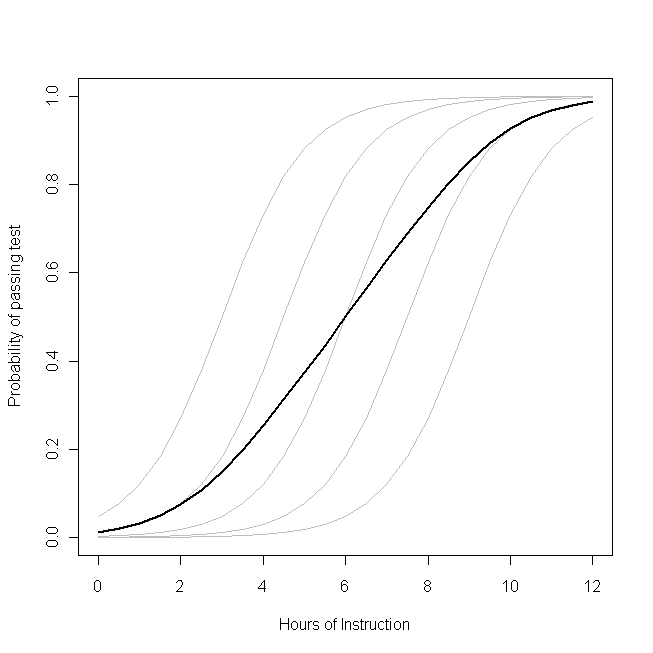
\includegraphics{fig/glmm_logit_StackOverflow.png}

Imagine that this plot represents the underlying data generating process for the probability that a small class of students will be able to pass a test on some subject with a given number of hours of instruction on that topic. Each of the grey curves represents the probability of passing the test with varying amounts of instruction for one of the students. The bold curve is the average over the whole class. In this case, the effect of an additional hour of teaching conditional on the student's attributes is β1\beta\_1--the same for each student (that is, there is not a random slope). Note, though, that the students baseline ability differs amongst them--probably due to differences in things like IQ (that is, there is a random intercept). The average probability for the class as a whole, however, follows a different profile than the students. The strikingly counter-intuitive result is this: an additional hour of instruction can have a sizable effect on the probability of each student passing the test, but have relatively little effect on the probable total proportion of students who pass. This is because some students might already have had a large chance of passing while others might still have little chance.

The question of whether you should use a GLMM or the GEE is the question of which of these functions you want to estimate. If you wanted to know about the probability of a given student passing (if, say, you were the student, or the student's parent), you want to use a GLMM. On the other hand, if you want to know about the effect on the population (if, for example, you were the teacher, or the principal), you would want to use the GEE.

\href{https://stats.stackexchange.com/questions/32419/difference-between-generalized-linear-models-generalized-linear-mixed-models}{StackOverFlow}

What are the best methods for checking a generalized linear mixed model (GLMM) for proper fit?
Unfortunately, it isn't as straightforward as it is for a general linear model.
n linear models the requirements are easy to outline: linear in the parameters, normally distributed and independent residuals, and homogeneity of variance (that is, similar variance at all values of all predictors).

For linear models, there are well-described and well-implemented methods for checking each of these, both visual/descriptive methods and statistical tests.

It is not nearly as easy for GLMMs.

\textbf{Assumption: Random effects come from a normal distribution}

Let's start with one of the more familiar elements of GLMMs, which is related to the random effects. There is an assumption that random effects---both intercepts and slopes---are normally distributed.

These are relatively easy to export to a data set in most statistical software (including SAS and R). Personally, I much prefer visual methods of checking for normal distributions, and typically go right to making histograms or normal probability plots (Q-Q plots) of each of the random effects.

If the histograms look roughly bell-shaped and symmetric, or the Q-Q plots generally fall close to a diagonal line, I usually consider this to be good enough.

If the random effects are not reasonably normally distributed, however, there are not simple remedies. In a general linear model outcomes can be transformed. In GLMMs they cannot.

Research is currently being conducted on the consequences of mis-specifying the distribution of random effects in GLMMs. (Outliers, of course, can be handled the same way as in generalized linear models---except that an entire random subject, as opposed to a single observation, may be examined.)

\textbf{Assumption: The chosen link function is appropriate}

Additional assumptions of GLMMs are more related to the generalized linear model side. One of these is the relationship of the numeric predictors to the parameter of interest, which is determined by the link function.

For both generalized linear models and GLMMs, it is important to understand that the most typical link functions (e.g., the logit for binomial data, the log for Poisson data) are not guaranteed to be a good representation of the relationship of the predictors with the outcomes.

Checking this assumption can become quite complicated as models become more crowded with fixed and random effects.

One relatively simple (though not perfect) way to approach this is to compare the predicted values to the actual outcomes.

With most GLMMs, it is best to compare averages of outcomes to predicted values. For example, with binomial models, one could take all of the values with predicted values near 0.5, 0.15, 0.25, etc., and average the actual outcomes (the 0s and 1s). You can then plot these average values against the predicted values.

If the general form of the model is correct, the differences between the predicted values and the averaged actual values will be small. (Of course how small depends on the number of observations and variance function).

No ``patterns'' in these differences should be obvious.

This is similar to the idea of the Hosmer-Lemeshow test for logistic regression models. If you suspect that the form of the link function is not correct, there are remedies. Possibilites include changing the link function, transforming numeric predictors, or (if necessary) categorizing continuous predictors.

\textbf{Assumption: Appropriate estimation of variance}

Finally, it is important to check the variability of the outcomes. This is also not as easy as it is for linear models, since the variance is not constant and is a function of the parameter being estimated.

Fortunately, this is one of the easier assumptions to check. One of the fit statistics your statistical software produces is a generalized chi-square that compares the magnitude of the model residuals to the theoretical variance.

The chi-square divided by its degrees of freedom should be approximately 1. If this statistic is too large, then the variance is ``overdispersed'' (larger than it should be). Alternatively, if the statistic is too small, the variance is ``underdispersed.''

While the best way to approach this varies by distribution, there are options to adjust models for overdispersion that result in more conservative p-values.

\href{https://www.theanalysisfactor.com/regression-diagnostics-glmm/}{TheAnalysisFactor}

\hypertarget{logit}{%
\section{Logit}\label{logit}}

Possible Analysis methods:

Below is a list of some analysis methods you may have encountered. Some of the methods listed are quite reasonable while others have either fallen out of favor or have limitations.

\begin{itemize}
\tightlist
\item
  Logistic regression, the focus of this page
\item
  Probit regression. Probit analysis will produce results similar logistic regression. The choice of probit versus logit depends largely on individual preferences.
\item
  OLS regression. When used with a binary response variable, this model is known as a linear probability model and can be used as a way to describe conditional probabilities. However, the errors (i.e., residuals) from the linear probability model violate the homoskedasticity and normality of errors assumptions of OLS regression, resulting in invalid standard errors and hypothesis tests. For a more thorough discussion of these and other problems with the linear probability model.
\item
  Two-group discriminant function analysis. A multivariate method for dichotomous outcome variables.
\item
  Hotelling's T2. The 0/1 outcome is turned into the grouping variable, and the former predictors are turned into outcome variables. This will produce an overall test of significance but will not give individual coefficients for each variable, and it is unclear the extent to which each ``predictor'' is adjusted for the impact of the other ``predictors.''
\end{itemize}

\href{https://stats.idre.ucla.edu/r/dae/logit-regression/}{ucla}

\hypertarget{odds-ratio}{%
\subsection{Odd's Ratio}\label{odds-ratio}}

If you want to interpret the estimated effects as relative odds ratios,
just do \texttt{exp(coef(x))} (gives you \(e^β\),
the multiplicative change in the odds ratio for \(y=1\)
if the covariate associated with \(β\) increases by 1).

For profile likelihood intervals for this quantity, you can do

\begin{verbatim}
require(MASS)
exp(cbind(coef(x), confint(x)))  
\end{verbatim}

To get the odds ratio, we need the classification cross-table
of the original dichotomous DV and
the predicted classification according to some probability threshold that needs to be chosen first.

\href{https://stats.stackexchange.com/questions/8661/logistic-regression-in-r-odds-ratio}{StackOverFlow}

\hypertarget{p-test}{%
\chapter{P test}\label{p-test}}

\hypertarget{p-value-hacking}{%
\section{P-Value Hacking}\label{p-value-hacking}}

Results from a study can be analyzed in a variety of ways, and p-hacking refers to a practice where researchers select the analysis that yields a pleasing result. The p refers to the p-value, a ridiculously complicated statistical entity that's essentially a measure of how surprising the results of a study would be if the effect you're looking for wasn't there.

P-hacking as a term came into use as psychology and some other fields of science were experiencing a kind of existential crisis. Seminal findings were failing to replicate. Absurd results (ESP is real!) were passing peer review at well-respected academic journals. Efforts were underway to test the literature for false positives and the results weren't looking good. Researchers began to realize that the problem might be woven into some long-standing and basic research practices

Exploiting what they called ``researcher degrees of freedom'': the little decisions that scientists make as they're designing a study and collecting and analyzing data. These choices include things like which observations to measure, which variables to compare, which factors to combine, and which ones to control for. Unless researchers have committed to a methodology and analysis plan in advance by preregistering a study, they are, in practice, free to make (or even change) these calls as they go.

This kind of fiddling around allows researchers to manipulate their study conditions until they get the answer that they want.

Even if you don't cheat, it's still a moral error to misanalyze data on a problem of consequence.

At its core, p-hacking is really about confirmation bias---the human tendency to seek and preferentially find evidence that confirms what we'd like to believe, while turning a blind eye to things that might contradict our preferred truths.

People in power don't understand the inevitability of p-hacking in the absence of safeguards against it.

We all p-hack, to some extent, every time we set out to understand the evidence in the world around us. If there's a takeaway here, it's that science is hard---and sometimes our human foibles make it even harder.

\href{https://www.wired.com/story/were-all-p-hacking-now/}{Wired}

Testing abused to create misleading results. This is a technique known colloquially as `p-hacking'. It is a misuse of data analysis to find patterns in data that can be presented as statistically significant when in fact there is no real underlying effect.

One of the most common ways in which data analysis is misused to generate statistically significant results where none exists, and is one which everyone reporting on science should remain vigilant against.

\href{https://scienceinthenewsroom.org/resources/statistical-p-hacking-explained/}{Statistical P-hacking explained}

\emph{Taleb}

We present the expected values from p-value hack-
ing as a choice of the minimum p-value among m independents
tests, which can be considerably lower than the ``true'' p-value,
even with a single trial, owing to the extreme skewness of the
meta-distribution.
We first present an exact probability distribution (meta-
distribution) for p-values across ensembles of statistically iden-
tical phenomena. We derive the distribution for small samples
2 \textless{} n ≤ n ∗ ≈ 30 as well as the limiting one as the sample size n
becomes large. We also look at the properties of the ``power'' of
a test through the distribution of its inverse for a given p-value
and parametrization.
The formulas allow the investigation of the stability of the
reproduction of results and ``p-hacking'' and other aspects of
meta-analysis.
P-values are shown to be extremely skewed and volatile,
regardless of the sample size n, and vary greatly across repetitions
of exactly same protocols under identical stochastic copies of the
phenomenon; such volatility makes the minimum p value diverge
significantly from the ``true'' one. Setting the power is shown to
offer little remedy unless sample size is increased markedly or
the p-value is lowered by at least one order of magnitude.

\href{pdf/Taleb_2018_P-Value-Hacking.pdf}{Taleb (2018) P-Value Hacling (pdf)}

\emph{Simmons}

In this article, we accomplish two things. First, we show that despite empirical psychologists' nominal endorsement of a low rate
of false-positive findings (≤ .05), flexibility in data collection, analysis, and reporting dramatically increases actual false-positive
rates. In many cases, a researcher is more likely to falsely find evidence that an effect exists than to correctly find evidence
that it does not. We present computer simulations and a pair of actual experiments that demonstrate how unacceptably easy
it is to accumulate (and report) statistically significant evidence for a false hypothesis. Second, we suggest a simple, low-cost,
and straightforwardly effective disclosure-based solution to this problem. The solution involves six concrete requirements for
authors and four guidelines for reviewers, all of which impose a minimal burden on the publication process.

\href{pdf/Simmons_2011_False_Positive_Psychology.pdf}{Simmons (2011) False positive psychology (pdf)}

\emph{Simonsohn}

Because scientists tend to report only studies (publication bias) or analyses (p-hacking) that ``work'', readers must ask, ``Are these effects true, or do they merely reflect selective reporting?'' We introduce p-curve as a way to answer this question. P-curve is the distribution of statistically significant p-values for a set of studies (ps \textless{} .05). Because only true effects are expected to generate right-skewed p-curves -- containing more low (.01s) than high (.04s) significant p-values -- only right-skewed p-curves are diagnostic of evidential value. By telling us whether we can rule out selective reporting as the sole explanation for a set of findings, p-curve offers a solution to the age-old inferential problems caused by file-drawers of failed studies and analyses.

\href{https://papers.ssrn.com/sol3/papers.cfm?abstract_id=2256237}{Simonsohn (2014) P-Curve}
\href{pdf/Simonsohm_2014_P-curve.pdf}{(pdf)}

\emph{Wikipedia}

Data dredging (or data fishing, data snooping, data butchery), also known as significance chasing, significance questing, selective inference, and p-hacking{[}1{]} is the misuse of data analysis to find patterns in data that can be presented as statistically significant, thus dramatically increasing and understating the risk of false positives. This is done by performing many statistical tests on the data and only reporting those that come back with significant results.

The process of data dredging involves testing multiple hypotheses using a single data set by exhaustively searching---perhaps for combinations of variables that might show a correlation, and perhaps for groups of cases or observations that show differences in their mean or in their breakdown by some other variable.

Conventional tests of statistical significance are based on the probability that a particular result would arise if chance alone were at work, and necessarily accept some risk of mistaken conclusions of a certain type (mistaken rejections of the null hypothesis). This level of risk is called the significance. When large numbers of tests are performed, some produce false results of this type; hence 5\% of randomly chosen hypotheses might be (erroneously) reported to be statistically significant at the 5\% significance level, 1\% might be (erroneously) reported to be statistically significant at the 1\% significance level, and so on, by chance alone. When enough hypotheses are tested, it is virtually certain that some will be reported to be statistically significant (even though this is misleading), since almost every data set with any degree of randomness is likely to contain (for example) some spurious correlations. If they are not cautious, researchers using data mining techniques can be easily misled by these results.

Data dredging is an example of disregarding the multiple comparisons problem. One form is when subgroups are compared without alerting the reader to the total number of subgroup comparisons examined.

\href{https://en.wikipedia.org/wiki/Data_dredging}{Wikipedia: Data dredging}

\emph{Head}

A focus on novel, confirmatory, and statistically significant results leads to substantial bias
in the scientific literature. One type of bias, known as ``p-hacking,'' occurs when researchers
collect or select data or statistical analyses until nonsignificant results become significant.
Here, we use text-mining to demonstrate that p-hacking is widespread throughout science.
We then illustrate how one can test for p-hacking when performing a meta-analysis and
show that, while p-hacking is probably common, its effect seems to be weak relative to the
real effect sizes being measured. This result suggests that p-hacking probably does not
drastically alter scientific consensuses drawn from meta-analyses.

\href{https://journals.plos.org/plosbiology/article?id=10.1371/journal.pbio.1002106}{Head (2015) Extent of P-Hacking}
\href{pdf/Head_2015_Extent_of_P-Hacking.pdf}{(pdf)}

\hypertarget{bootstrapping-instead-of-p-values}{%
\section{Bootstrapping instead of p-values}\label{bootstrapping-instead-of-p-values}}

\emph{Buisson}

P-values don't mean what people think they mean; they rely on hidden assumptions that are unlikely to be fulfilled; they detract from the real questions. Here's how to use the Bootstrap in R and Python instead

There are many reasons why you should abandon p-values, and I'll examine three of the main ones here:

\begin{verbatim}
They don’t mean what people think they mean

They rely on hidden assumptions that are unlikely to be fulfilled

They detract from the real questions
\end{verbatim}

\href{https://towardsdatascience.com/ditch-p-values-use-bootstrap-confidence-intervals-instead-bba56322b522}{Buisson (2021) Ditch p-values. Use Bootstrap confidence intervals instead}

\hypertarget{probit}{%
\section{Probit}\label{probit}}

A standard linear model (e.g., a simple regression model) can be thought of as having two `parts'.
These are called the structural component and the random component.
For example:

\[Y=β_0+β_1 X+ε\]

where

\(ε∼N(0,σ^2)\)

The first two terms (that is, \(β_0 + β_1 X\)) constitute the structural component,
and the \(ε\) (which indicates a normally distributed error term) is the random component.

When the response variable is not normally distributed
(for example, if your response variable is binary) this approach may no longer be valid.

The generalized linear model (GLiM) was developed to address such cases,
and logit and probit models are special cases of GLiMs that are appropriate for binary variables
(or multi-category response variables with some adaptations to the process).

A GLiM has three parts, a \emph{structural component}, a \emph{link function}, and a \emph{response distribution}.

For example:

\[g(μ)=β_0+β_1 X\]

Here \(β_0 + β_1 X\) is again the structural component, \(g()\) is the link function,
and \(μ\) is a mean of a conditional response distribution at a given point in the covariate space.

The way we think about the structural component here doesn't really differ from how we think about it
with standard linear models; in fact, that's one of the great advantages of GLiMs.
Because for many distributions the variance is a function of the mean,
having fit a conditional mean (and given that you stipulated a response distribution),
you have automatically accounted for the analog of the random component in a linear model
(N.B.: this can be more complicated in practice).

The link function is the key to GLiMs:
since the distribution of the response variable is non-normal,
it's what lets us connect the structural component to the response--
it `links' them (hence the name).
It's also the key to your question, since the logit and probit are links,
and understanding link functions will allow us to intelligently choose when to use which one.
Although there can be many link functions that can be acceptable,
often there is one that is special.
Without wanting to get too far into the weeds (this can get very technical) the predicted mean, \(μ\),
will not necessarily be mathematically the same as
the response distribution's canonical location parameter;
the link function that does equate them is the canonical link function.
The advantage of this "is that a minimal sufficient statistic for \(β\).
The canonical link for binary response data (more specifically, the binomial distribution) is the logit.
However, there are lots of functions that can map the structural component onto the interval (0,1)(0,1),
and thus be acceptable; the probit is also popular, but there are yet
other options that are sometimes used (such as the \emph{complementary log log}, \(ln(−ln(1−μ))\),
often called \emph{cloglog}).
Thus, there are lots of possible link functions and
the choice of link function can be very important.
The choice should be made based on some combination of:

\begin{enumerate}
\def\labelenumi{\arabic{enumi}.}
\tightlist
\item
  Knowledge of the response distribution,
\item
  Theoretical considerations, and
\item
  Empirical fit to the data.
\end{enumerate}

These considerations can be used to guide your choice of link.
To start with, if your response variable is the outcome of a Bernoulli trial (that is, 0 or 1),
your response distribution will be binomial,
and what you are actually modeling is the probability of an observation being a 1
(that is, \(π(Y=1)\).
As a result, any function that maps the real number line, \((−∞,+∞)\)
to the interval \((0,1)\) will work.

If you are thinking of your covariates as directly connected to the probability of success,
then you would typically choose logistic regression
because it is the canonical link.
However, consider the following example:
You are asked to model high\_Blood\_Pressure as a function of some covariates.
Blood pressure itself is normally distributed in the population.
Clinicians dichotomized it during the study
(that is, they only recorded `high-BP' or `normal').
In this case, probit would be preferable a-priori for theoretical reasons.
Your binary outcome depends on a hidden Gaussian variable.
Another consideration is that both logit and probit are symmetrical,
if you believe that the probability of success rises slowly from zero,
but then tapers off more quickly as it approaches one, the cloglog is called for.

Lastly, note that the empirical fit of the model to the data is
unlikely to be of assistance in selecting a link,
unless the shapes of the link functions in question differ substantially
(of which, the logit and probit do not).
For instance, consider the following simulation:

\begin{verbatim}
set.seed(1)
probLower = vector(length=1000)

for(i in 1:1000){      
    x = rnorm(1000)
    y = rbinom(n=1000, size=1, prob=pnorm(x))

    logitModel  = glm(y~x, family=binomial(link="logit"))
    probitModel = glm(y~x, family=binomial(link="probit"))

    probLower[i] = deviance(probitModel)<deviance(logitModel)
}

sum(probLower)/1000
[1] 0.695
\end{verbatim}

Even when we know the data were generated by a probit model, and we have 1000 data points,
the probit model only yields a better fit 70\% of the time, and even then,
often by only a trivial amount.
Consider the last iteration:

\begin{verbatim}
deviance(probitModel)
[1] 1025.759
deviance(logitModel)
[1] 1026.366
deviance(logitModel)-deviance(probitModel)
[1] 0.6076806
\end{verbatim}

The reason for this is simply that the logit and probit link functions
yield very similar outputs when given the same inputs.

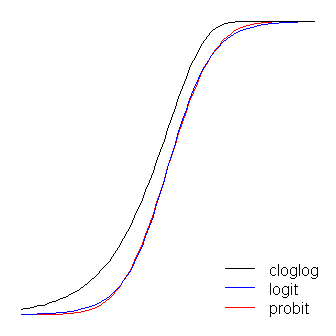
\includegraphics{fig/glmm_probit_StackOverflow.png}

The logit and probit functions are practically identical,
except that the logit is slightly further from the bounds when they `turn the corner'.
(Note that to get the logit and the probit to align optimally,
the logit's \(β_1\) must be \(≈1.7\) times the corresponding slope value for the probit.
In addition, I could have shifted the cloglog over slightly
so that they would lay on top of each other more,
but I left it to the side to keep the figure more readable.
Notice that the cloglog is asymmetrical whereas the others are not;
it starts pulling away from 0 earlier, but more slowly,
and approaches close to 1 and then turns sharply.

A couple more things can be said about link functions.
First, considering the \emph{identity function} \((g(η)=ηg(\eta)=\eta)\)
as a link function allows us to understand the standard linear model
as a special case of the generalized linear model
(that is, the response distribution is normal, and the link is the identity function).
It's also important to recognize that whatever transformation the link instantiates
is properly applied to the parameter governing the response distribution (that is, \(μ\)),
not the actual response data.
Finally, because in practice we never have the underlying parameter to transform,
in discussions of these models,
often what is considered to be the actual link is left implicit and
the model is represented by the inverse of the link function
applied to the structural component instead.
That is:

\[μ=g^{−1}(β_0+β_1 X)\]

For instance, logistic regression is usually represented:

\[π(Y)=\frac{exp(β_0 + β_1 X)}{1+exp(β_0 + β_1 X)}\]

instead of:

\[ln(\frac{(π(Y)}{1−π(Y)}) = β_0 + β_1 X\]

For a quick and clear, but solid, overview of the generalized linear model,
see chapter 10 of Fitzmaurice, Laird, \& Ware (2004),
For how to fit these models in R, check out the documentation for the function ?glm in the base package.

(One final note added later:) I occasionally hear people say that
you shouldn't use the probit, because it can't be interpreted.
This is not true, although the interpretation of the betas is less intuitive.
With logistic regression, a one unit change in \(X_1\) is associated with
a \(β_1\) change in the log odds of `success'
(alternatively, an \(exp(β_1)\)-fold change in the odds), all else being equal.
With a probit, this would be a change of \(β_1 z\)'s.
(Think of two observations in a dataset with \(z\)-scores of 1 and 2, for example.)
To convert these into predicted \emph{probabilities},
you can pass them through the normal CDF, or look them up on a \(z\)-table.

\href{https://stats.stackexchange.com/questions/20523/difference-between-logit-and-probit-models/30909\#30909}{StackOverFlow}

\hypertarget{spurious-correlation}{%
\chapter{Spurious Correlation}\label{spurious-correlation}}

\hypertarget{trending-variables}{%
\section{Trending Variables}\label{trending-variables}}

\emph{Tambonthongchai}

THE SOURCE DATA SHOW A STRONG STATISTICALLY SIGNIFICANT CORRELATION OF CORR=0.75 BETWEEN ANNUAL CHANGES IN MLO CO2 AND ANNUAL EMISSIONS. THIS CORRELATION APPEARS TO SUPPORT THE USUAL ASSUMPTION THAT CHANGES IN ATMOSPHERIC CO2 CONCENTRATION ARE CAUSED BY FOSSIL FUEL EMISSIONS AND THAT THEREFORE THESE CHANGES CAN BE MODERATED WITH CLIMATE ACTION TO CONTROL AND REDUCE THE RATE OF WARMING.

HOWEVER, IT IS KNOWN THAT SOURCE DATA CORRELATION BETWEEN TIME SERIES DATA DERIVE FROM TWO SOURCES. THESE ARE (1) SHARED TRENDS WITH NO CAUSATION IMPLICATION AND (2) RESPONSIVENESS AT THE TIME SCALE OF INTEREST. HERE THE TIME SCALE OF INTEREST IS ANNUAL BECAUSE THE THEORY REQUIRES THAT ANNUAL CHANGES IN ATMOSPHERIC CO2 CONCENTRATION ARE CAUSED BY ANNUAL FOSSIL FUEL EMISSIONS. THIS TEST IS MADE BY REMOVING THE SHARED TREND THAT IS KNOWN TO HAVE NO CAUSATION INFORMATION OR IMPLICATION. HERE WE FIND THAT WHEN THE SHARED TREND IS REMOVED THE OBSERVED CORRELATION DISAPPPEARS. THE APPARENT CORRELATION BETWEEN EMISSIONS AND CHANGES IN ATMOSPHERIC CO2 CONCENTRATION IS THUS FOUND TO BE SPURIOUS.

THE DATA FOR ANNUAL FOSSIL FUEL EMISSIONS AND ANNUAL CHANGES IN ATMOSPHERIC CO2 CONCENTRATION DO NOT SHOW THAT FOSSIL FUEL EMISSIONS CAUSE ATMOSPHERIC CO2 CONCENTRATION TO CHANGE. THE FINDING IMPLIES THAT THERE IS NO EMPIRICAL EVIDENCE IN SUPPORT OF THE THEORY OF CLIMATE ACTION. THIS THEORY HOLDS THAT MOVING THE GLOBAL ENERGY INFRASTRUCTURE FROM FOSSIL FUELS TO RENEWABLES WILL MODERATE THE RATE OF INCREASE IN ATMOSPHERIC CO2 AND THEREBY MODERATE THE RATE OF WARMING.

\href{https://tambonthongchai.com/2020/11/11/annual-changes-in-mlo-co2/}{Tambonthongchai: Climate Data Case (via Arve)}

\emph{Munshi Abstract}

\textbf{Abstract:} Unrelated time series data can show spurious correlations by virtue of a shared drift in the long term trend. The
spuriousness of such correlations is demonstrated with examples. The SP500 stock market index, GDP at current prices for the
USA, and the number of homicides in England and Wales in the sample period 1968 to 2002 are used for this demonstration.
Detrended analysis shows the expected result that at an annual time scale the GDP and SP500 series are related and that
neither of these time series is related to the homicide series. Correlations between the source data and those between
cumulative values show spurious correlations of the two financial time series with the homicide series.
These results have implications for empirical evidence that attributes changes in temperature and carbon dioxide levels in the surface-atmosphere system to fossil fuel emissions

\emph{Munshi Memo}

Spurious correlations of this nature are sometimes found in published research. For example, climate
science attributes the rise in atmospheric carbon dioxide to fossil fuel emissions and cites correlations
between the data as empirical evidence (IPCC, 2007) (IPCC, 2014) (Canadell, 2007) (Kheshgi, 2005).
Detrended analysis shows that correlations between emissions and atmospheric CO2 and oceanic CO2
are spurious because they disappear when the data are detrended (Munshi, Responsiveness of
Atmospheric CO2 to Anthropogenic Emissions, 2015) (Munshi, Fossil Fuel Emissions and Ocean
Acidification, 2015). These anomalous results likely derive from large and perhaps unquantifiable
uncertainties in natural flows of carbon dioxide in the surface-atmosphere system (Munshi, Uncertain
Flow Accounting and the IPCC Carbon Budget, 2015).

\href{https://www.researchgate.net/publication/306376553_Spurious_Correlations_in_Time_Series_Data_A_Note}{Munshi (2016) Spurious Correlations in Time Series Data: A Note}
{[}(pdf){[}pdf/Munshi\_2016\_Spurious\_Time\_Series.pdf)

\emph{Munshi Abstract}

A statistically significant correlation between annual anthropogenic CO2 emissions and the annual rate of accumulation of CO2 in the atmosphere over a 53-year sample period from 1959-2011 is likely to be spurious because it vanishes when the two series are detrended. The results do not indicate a measurable year to year effect of annual anthropogenic emissions on the annual rate of CO2 accumulation in the atmosphere.

\href{https://papers.ssrn.com/sol3/papers.cfm?abstract_id=2642639}{Munshi 82015) Spurious Anthropogenic CO2}
\href{pdf/Munshi_2015_Spurious_Antropogenic_CO2.pdf}{(pdf)}

\emph{Wu Abstract}

This paper examines three types of spurious regressions where both the dependent and
independent variables contain deterministic trends, stochastic trends, or breaking trends. We
show that the problem of spurious regression disappears if the trend functions are included as
additional regressors. In the presence of autocorrelation, we show that using a Feasible General
Least Square (FGLS) estimator can help alleviate or eliminate the problem. Our theoretical
results are clearly reflected in finite samples. As an illustration, we apply our methods to revisit
the seminal study of Yule (1926).

\href{pdf/Wu_2007_Spurious_Trending.pdf}{Wu (2007) On spurious regressions with trending variables (pdf)}

\hypertarget{stationarity}{%
\chapter{Stationarity}\label{stationarity}}

\hypertarget{record-events}{%
\section{Record Events}\label{record-events}}

Whenever there is a new record-breaking weather event, such as record-high temperatures, it is natural to ask whether the occurrence of such an event is due to a climate change. Before we proceed, it may be useful to define the term `statistically stationary', the meaning here being that statistical aspects of the weather (means, standard deviation etc.) aren't changing. In statistics, there is a large volume of literature on record-breaking behaviour, and statistically stationary systems will produce new record-breaking events from time to time. On the other hand, one would expect to see more new record-breaking events in a changing climate: when the mean temperature level rises new temperatures will surpass past record-highs.

\href{https://www.realclimate.org/index.php/archives/2005/08/on-record-high-temperatures/}{Benestad (2005) On record-breaking events (RealClimate.org)}

*Abstract Benestad)

This study applies a simple framework for analysing the incidence of record events. A
test of this method on the global mean temperature yields results consistent with a global warming,
where record-warm events are more frequent than for a stationary series. The record event analysis
suggests that the number of record-warm monthly global mean temperatures is higher than
expected, and that the number of record events in the absolute monthly maximum and minimum
temperatures in the Nordic countries is slightly higher than expected from a null hypothesis of a sta-
tionary behaviour. Because the different station series are not strictly independent, it is difficult to
resolve whether there is a significant trend in the warmest absolute monthly minimum temperatures
in the Nordic countries. The behaviour of the maximum monthly 24 h precipitation is not distin-
guishable from the null hypothesis that the series consists of independent and identically distributed
random variables.

\href{pdf/Benestad_2003_How_often_record_event.pdf}{Benestad (2003) How often can we expect a record event? (Climate Resarch) (pdf)}

\hypertarget{power-laws}{%
\chapter{Power laws}\label{power-laws}}

\begin{quote}
Recent advances in
network science show that many growing associations -- including those whose evolution is
often thought of as spontaneous and voluntary, from the internet and World Wide Web, to
aviation routes and NGO ties, to production chains, academic publications and terrorist organ-
izations -- end up developing into so-called scale-free networks. The term `scale-free' here in-
dicates that the size of the nodes, measured by the number of their connections, does not have
`typical' scale. Instead of following a bell-shaped distribution, it obeys power laws, with a small
number of very large hubs dominating a countless mass of smaller nodes. So here too we have
hierarchy. (Bichler \& Nitzan (2021) Growing through Sabotage)
\end{quote}

\hypertarget{generative-models}{%
\section{Generative Models}\label{generative-models}}

\emph{Mitzenmacher Abstract}

Recently, I became interested in a current debate over whether file size
distributions are best modelled by a power law distribution or a lognormal distribution.
In trying to learn enough about these distributions to settle the question, I found a rich
and long history, spanning many fields. Indeed, several recently proposed models from
the computer science community have antecedents in work from decades ago. Here,
I briefly survey some of this history, focusing on underlying generative models that
lead to these distributions. One finding is that lognormal and power law distributions
connect quite naturally, and hence, it is not surprising that lognormal distributions
have arisen as a possible alternative to power law distributions across many fields.

\emph{Mitzenmacher Memo}

\href{pdf/Mitzenmacher_2004_Generative_Models_Power_Law.pdf}{Mitzenmacher(2004) A Brief History of Generative Models for Power Law and Lognormal Distributions (pdf)}

\hypertarget{income-distribution-power-law}{%
\section{Income Distribution Power Law}\label{income-distribution-power-law}}

\emph{Fix Abstract}

Although the determinants of income are complex, the results are surprisingly uniform. To a first approximation, top incomes follow a power-law distribution, and the redistribution of income corresponds to a change in the power-law exponent. Given the messiness of the struggle for resources, why is the outcome so simple?

This paper explores the idea that the (re)distribution of top incomes is uniform because it is shaped by a ubiquitous feature of social life, namely hierarchy. Using a model first developed by Herbert Simon and Harold Lydall, I show that hierarchy can explain the power-law distribution of top incomes, including how income gets redistributed as the rich get richer.

\emph{Fix Memo}

Although the causal mechanisms may appear complex, the mathematical mechanisms for generating power laws are surprisingly simple. I will discuss two main routes. (For a review of mechanisms for generating power laws, see Mitzenmacher, 2004.)

The first route to a power law is through income dynamics. Suppose an individual starts out with annual income I . Over time, their income grows and shrinks for reasons that we do not understand. But what we do know is that this income change can be modelled as a random number. After t years, the person's new income is the product of successive random growth rates, g :

\(I_t = I_1 * g_1 * g_2 * ... * g_t\)

Now suppose that everyone's income behaves the same way: it is the product of a series of random growth rates. After many growth iterations, the resulting distribution of income will follow a lognormal distribution --- a fact discovered by Robert Gibrat (\href{https://economicsfromthetopdown.com/2021/10/24/redistributing-income-through-hierarchy/\#ref-gibrat_les_1931}{1931}).

To get a power-law distribution, we introduce one more requirement: a lower `wall' that limits the smallness of incomes. If anyone's income gets below this lower threshold, it gets `reflected' in the opposite direction. After many growth iterations, income will be distributed according to a power law.

This `stochastic' model of income was first articulated by David Champernowne (\href{https://economicsfromthetopdown.com/2021/10/24/redistributing-income-through-hierarchy/\#ref-champernowne_model_1953}{1953}). While the model's mathematics are beyond dispute, many political economists find its appeal to `randomness' troubling. After all, incomes have definite causes (or so we believe). But to be fair to the Champernowne model, it does not claim that income dynamics are actually random, only that we can model them as such.

The Champernowne model tells us that we can understand the power-law distribution of top incomes without knowing anything about the complexities of human behavior. All that we need are general assumptions about the dynamics of income. I find this result fascinating because it is counter-intuitive. Yet it is also underwhelming because it does not tell us why people earn what they do. For that reason, I will focus on a second route to power laws --- a route that can be tied to social structure.

The second route to a power law comes from merging two different exponential functions. Suppose two variables, \(x\) and \(y\) , are both exponential functions of a third variable, \(t\) :

\[x = e^{a*t}\]

\[y = e^{b*t}\]

If we combine these two functions and eliminate t , we find that x and y are related by a power law:

\[y = x ^{b/a}\]

So we can create a power law by merging two exponential functions.
The question is, why would such functions apply to income?
The answer, I propose, is simple.
These are the equations that describe income in a hierarchy.

Because Simon and Lydall's pioneering research was completed a half century ago, one would think that today there would be a burgeoning literature on the distributional consequences of hierarchy. Sadly, this is not the case. Instead, shortly after Simon and Lydall published their work, the study of income distribution became dominated by human capital theory, which focused on personal traits and neglected `structural' explanations of income.

Treating CEOs as canaries in the coal mine. I propose that the exploding pay of CEOs is part of a wider redistribution of income within hierarchies. It is evidence that US firms are becoming more \emph{despotic}:
Rulers can use their power to benefit the group. But they can also use their power to enrich themselves. The more they do so, the more `\emph{despotic}' the hierarchy.
The more despotic the hierarchy becomes, the more rapidly income will increase with hierarchical power.

It makes sense, then, to use the scaling of income with hierarchical power, D , as a measure of the `degree of hierarchical despotism'. The greater the value of D , the more despotic the hierarchy.

\[relative income \propto (hierarchical power)^D\]

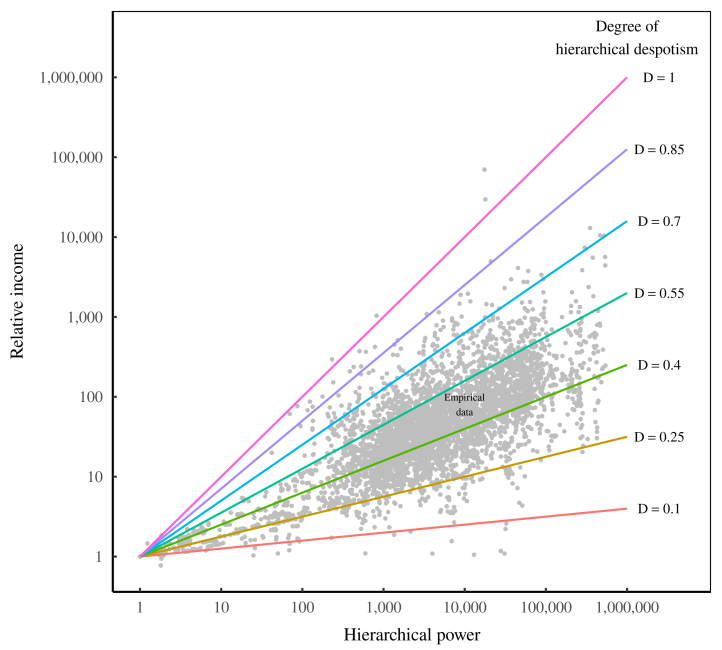
\includegraphics{fig/despotism_diagram.png}

In large hierarchies, the value of \(D\) affects top incomes dramatically. For instance, when \(D=0.1\) , a CEO with one million subordinates will earn only about 4 times more than a bottom-ranked worker. But when \(D=1\) , the same CEO will earn a million times more than an entry-level employee.

\href{https://economicsfromthetopdown.com/2021/10/24/redistributing-income-through-hierarchy/}{Fix (2021) Redistributing Income Through Hierarchy}

\hypertarget{timescaling-rainfall}{%
\section{Timescaling Rainfall}\label{timescaling-rainfall}}

\emph{Abstract Benestad}

Abstract
A simple formula for estimating approximate values of return levels for sub-daily rainfall is
presented and tested. It was derived from a combination of simple mathematical principles,
approximations and fitted to 10 year return levels taken from intensity-duration-frequency (IDF)
curves representing 14 sites in Oslo. The formula was subsequently evaluated against IDF curves
from independent sites elsewhere in Norway. Since it only needs 24 h rain gauge data as input, it
can provide approximate estimates for the IDF curves used to describe sub-daily rainfall return
levels. In this respect, it can be considered as means of downscaling with respect to timescale, given
an approximate power-law dependency between temporal scales. One clear benefit with this
framework is that observational data is far more abundant for 24 h rain gauge records than for
sub-daily measurements. Furthermore, it does not assume stationarity, and is well-suited for
projecting IDF curves for a future climate.

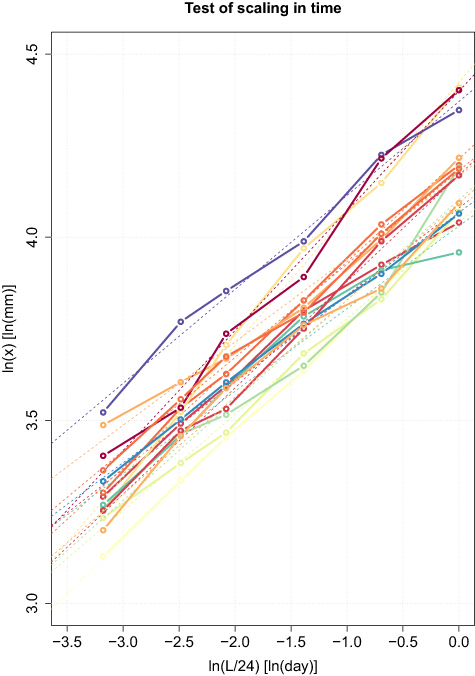
\includegraphics{fig/Benestad_Timescaling.jpg}

\href{https://iopscience.iop.org/article/10.1088/1748-9326/abd4ab}{Benestad (2021) Intensity-Duration-frequency Rainfall}
\href{pdf/Benestad_2021_Intensity_Duration_Frequency.pdf}{(pdf)}

\hypertarget{syntetic-control}{%
\chapter{Syntetic Control}\label{syntetic-control}}

\textbf{Testing Washington Consensus}

A true assessment of the Washington Consensus, however, requires a sharply formed counterfactual: Did countries that embraced policy reforms do better than those that either chose not to reform or chose a different path? Having a well-defined counterfactual is a necessary part of any ex post evaluation of a particular policy regime.

In a recent article in the Journal of Comparative Economics, ``\href{https://www.sciencedirect.com/science/article/pii/S0147596720300639}{The Washington Consensus Works: Causal Effects of Reform, 1970-2015},'' Kevin Grier and Robin Grier find that countries undertaking sustained economic reform had a 16 percent higher real per capita GDP after 10 years, compared to other countries.

Another recent paper, by Marco Marrazzo and Alessio Terzi, \href{https://papers.ssrn.com/sol3/papers.cfm?abstract_id=3071545}{Structural Reform Waves and Economic Growth}, finds that the benefits of structural reform are smaller (6 percent of GDP compared to a counterfactual) and appear after five years

Both papers explicitly consider a counterfactual. Grier and Grier compare countries undergoing large and sustained increases in an index of economic freedom (as well as those with large and sustained decreases) to countries undertaking few or no changes in policy stance. Marrazzo and Terzi use synthetic control methods to compare the growth trajectories of reforming and very similar non-reforming countries.

An alternative approach would be to consider the antithesis of Washington Consensus--type policies, such as those associated with economic populism.{[}5{]} Such policies include economic nationalism (trade and investment protectionism), large expansions in fiscal deficit spending, and greater state control over industry. An October 2020 study by Manuel Funke, Moritz Schularick, and Christoph Trebesch on ``\href{https://t.co/R5qYmjA3I8?amp=1}{Populist Leaders and the Economy}'' finds a huge economic cost to populist policies.
Looking at the record of 50 populist leaders over the period 1900--2018, they find that real GDP per capita is 10 percent lower after 15 years compared to a plausible non-populist leader counterfactual. They also find that inequality fails to decline under populist rule.

Similarly, in ``\href{https://www.sciencedirect.com/science/article/pii/S0167268120302237}{The Economic Consequences of Durable Left-Populist Regimes in Latin America},'' published in the September 2020 issue of the Journal of Economic Behavior and Organization, Samuel Absher, Kevin Grier, and Robin Grier find that left-wing populism made Venezuela, Nicaragua, and Bolivia 20 percent poorer relative to a plausible counterfactual. These countries did not experience reduced inequality or improved health outcomes that might have justified such a large sacrifice of income.

\href{https://www.piie.com/blogs/realtime-economic-issues-watch/washington-consensus-stands-test-time-better-populist-policies}{Peterson Inst: Populism Wash Consensus}

\href{https://en.wikipedia.org/wiki/Synthetic_control_method}{Wikipedia}

\href{pdf/Abadie_Synthetic_Control_Methods.pdf}{Abadie: Syntetic Control Methods (pdf)}

\href{pdf/Abadie_Using_Synthetic_Controls.pdf}{Abadie: Using Syntetic Controls (pdf)}

\hypertarget{econometrics}{%
\chapter{Econometrics}\label{econometrics}}

\emph{Goldsmith-Pinkham}

\textbf{Gary Chamberlain}

This document contains the set of lecture notes from the late Gary Chamberlain's 2010 Econometrics class (EC2120) that I (Paul Goldsmith-Pinkham) took during my economics Ph.D.~at Harvard University. Gary was a remarkable teacher and this class was an amazing experience for me as a young economist.

A few things worth noting from my experience taking this course:

\begin{verbatim}
The course is somewhat unique in not introducing any inference until Lecture 7 (halfway through the course). The focus prior to this is exclusively on estimation using regression.
The lectures are linked together in groups (even though they are not marked this way). Lectures 1-3 reflect the underlying setup in notation and framework for the rest of the course. Lectures 6-9 setup inference. Lecture 9-11 discuss a general framework for using moment conditions.
During my semester, we never got through lectures 13-15, which suggests that this is a lot of material for a single semester.
Gary would continually refer back to Lecture 4 and Lecture 9 (indeed, I have Gary's voice saying "if we think back to the Note 9 framework..." burned into my brain. As a result, these are also some of the longest and densest lectures.
The last 4 sections are review problems that Gary provided for preparation for the final exam. These are very fun problems, but we were not provided solutions. So, you'll have to figure them out on your own!
\end{verbatim}

\href{https://github.com/paulgp/GaryChamberlainLectureNotes}{Chamberlain Lecture Notes (Github)}

\hypertarget{part-appendices}{%
\part{Appendices}\label{part-appendices}}

\hypertarget{appendix-appendices}{%
\appendix}


\hypertarget{about}{%
\chapter{About}\label{about}}


\includegraphics{fig/me.jpg}

\emph{Dyre Haugen} and \emph{Dyrehaugen} is Webian for \emph{Jon Martin} -
self-owned Globian, Webian, Norwegian and Canarian with
a background from industrial research policy, urban planning and
economic development consulting on global, regional and urban scales.
I am deeply concerned about the (insane) way
humanity (i.e.~capitalism) interfere with nature.
In an effort to gain insights in how and why this happens
stuff is collected from around the web and put together
in a linked set of web-sites.
The sites are operated as personal notebooks.
However, these days things can be easily published to the
benefit of others concerned with the same issues.
But be aware - this is not polished for presentation or
peer-reviewed for exactness.
I offer you just to have a look at my `work-desk' as it appears in the moment.
Any comment or suggestion can be mailed to \href{mailto:dyrehaugen@gmail.com}{\nolinkurl{dyrehaugen@gmail.com}}
You can follow me on twitter as @dyrehaugen.
Thanks for visiting!

\hypertarget{links}{%
\chapter{Links}\label{links}}

\textbf{Current Dyrehaugen Sites:}

\begin{itemize}
\tightlist
\item
  \href{https://dyrehaugen.github.io/rcap}{rcap - On Capitalism} \href{http://localhost/rcap}{(loc)}
\item
  \href{https://dyrehaugen.github.io/rclm}{rclm - On Climate Change} \href{http://localhost/rclm}{(loc)}
\item
  \href{https://dyrehaugen.github.io/recs}{recs - On Economics} \href{http://localhost/recs}{(loc)}
\item
  \href{https://dyrehaugen.github.io/rngy}{rfin - On Finance} \href{http://localhost/rfin}{(loc)}
\item
  \href{https://dyrehaugen.github.io/rngy}{rngy - On Energy} \href{http://localhost/rngy}{(loc)}
\item
  \href{https://dyrehaugen.github.io/renv}{renv - On Environment} \href{http://localhost/renv}{(loc)}
\item
  \href{https://dyrehaugen.github.io/rsts}{rsts - On Statistics} \href{http://localhost/rsts}{(loc)}
\item
  \href{https://dyrehaugen.github.io/rurb}{rurb - On Urbanization} \href{http://localhost/rurb}{(loc)}
\item
  \href{https://dyrehaugen.github.io/rvar}{rvar - On Varia} \href{http://localhost/rvar}{(loc)}
\item
  \href{https://dyrehaugen.github.io/rwsd}{rwsd - On Wisdom} \href{http://localhost/rwsd}{(loc)}
\end{itemize}

\textbf{Blogs:}

\begin{itemize}
\tightlist
\item
  \href{https://dyrehaugen.github.io/rde}{rde - Blog in English} \href{http://localhost/rde}{(loc)}
\item
  \href{https://dyrehaugen.github.io/rdn}{rdn - Blog in Norwegian} \href{http://localhost/rdn}{(loc)}
\end{itemize}

\textbf{Discontinued:}

\begin{itemize}
\tightlist
\item
  \href{https://dyrehaugen.github.io/jdt}{jdt - Collection (Jekyll)} \href{http://localhost/jdt}{(loc)}
\item
  \href{https://dyrehaugen.github.io/hdt}{hdt - Collection (Hugo)} \href{http://localhost/hdt}{(loc)}
\end{itemize}

\textbf{Not listed:}

\begin{itemize}
\tightlist
\item
  (q:) dhe dhn jrw56
\item
  (z:) rcsa rpad rstart
\end{itemize}

\hypertarget{news}{%
\chapter{NEWS}\label{news}}

  \bibliography{book.bib,packages.bib}

\end{document}
